% =========================================================================
% 《高中數學實驗教材》第四冊（自然組）
% 第四章 二次幾何 第三部分：二次曲線的分類與判別
% =========================================================================

\section{二次幾何\texorpdfstring{\quad }{ }第三部分：二次曲線的分類與判別}
\label{sec:b4-ch4}

\begin{center}
\begin{minipage}{0.75\textwidth}
\begin{itemize}[leftmargin=2em, itemsep=0.3em]
  \item[§ IV-1] \textbf{二次曲線與其特異性}
  \item[§ IV-2] \textbf{固有值理論}
  \begin{itemize}[leftmargin=2em, itemsep=0.2em]
    \item[甲、] 問題的分析
    \item[乙、] 固有值與固有向量的求法
  \end{itemize}
  \item[§ IV-3] \textbf{二次式的標準化}
  \item[§ IV-4] \textbf{不變量}
  \begin{itemize}[leftmargin=2em, itemsep=0.2em]
    \item[甲、] 空間的二次幾何
    \item[乙、] 二元二次函數與剛性座標變換
  \end{itemize}
  \item[§ IV-5] \textbf{二次曲線的分類}
  \item[*§ IV-6] \textbf{五點決定一個二次曲線}
  \item[*§ IV-7] \textbf{圓錐面與錐線的再處理}
  \begin{itemize}[leftmargin=2em, itemsep=0.2em]
    \item[甲、] 從截面來判別錐線類型
    \item[乙、] 截痕為二次曲線的直接驗證
  \end{itemize}
\end{itemize}
\end{minipage}
\end{center}

\begin{center}
$* \qquad * \qquad * \qquad * \qquad *$
\end{center}

這是二次幾何的最後一章，進入二次幾何較深刻的主題．我們在第三章看出橢圓，拋物線，雙曲線都是二次曲線，但是，是否所有二次曲線都是這三種錐線之一？

§ IV-1 提出一些特異的情形，利用不變量 $\delta, \Delta, H$ 把牠們分濾出去，為分類定理舖路\phantomsection\label{note:b4-ch4-intro-pulu}\footnote{【原書註記/校訂】：原書目錄頁底文字與第 185 頁接續．原書排印「利用不變量，$\delta$，$\Delta$ 把牠們分濾出去」，依正文符號校訂為不變量 $\delta, \Delta, H$．}．然後，我們的分類定理便說所有非特異的二次曲線必為橢圓，拋物線，雙曲線三者之一\phantomsection\label{note:b4-ch4-intro-sanzhe}\footnote{【原書註記/校訂】：原書此處印作「三煮之」，顯係「三者之一」之排版訛字，茲予校訂．}．這一樁舖路工作的另一目的在於澄清 $\Delta$ 這一怪物的涵意\phantomsection\label{note:b4-ch4-intro-guaiwu}\footnote{【原書註記/校訂】：原書印作「這一径物」，字模殘損，依文義校訂為「怪物」．}．

在分類過程中，我們一反傳統改以發展固有值理論這一近代數學的重要工具來代替記憶轉軸公式，我們的目的有兩層：一來固有值理論本身含意頗長，深值學習；二來處理二次曲線的方法實際上脈絡清晰，不必死記．

然後是一般二次曲線的判別問題，早在 § IV-1 末，我們便以圖解，預先整理了判別的標準．

摻合在分類定理的導引過程中，一些二元二次函數在空間中所代表的簡單圖形也被提出（§ IV-4）．

§ IV-6 中三點決定一圓，四點決定一拋物線，五點決定一個一般二次曲線的討論，相當程度又與自由度有著關聯（注意：一點換算為一個（度）自由度）．最後，§ IV-7 是第二章部分內容的再處理，此處我們利用向量與座標幾何來驗證第二、三章的結果，同時藉此熟習空間中向量與座標幾何的運算．


\subsection{§ IV-1\texorpdfstring{\quad }{ }二次曲線與其特異性}

一個二元二次方程式的一般式為
\begin{equation}
Ax^2 + 2Bxy + Cy^2 + 2Dx + 2Ey + F = 0
\label{eq:b4-ch4-general-conic}
\end{equation}
式中二次項 $x^2, xy, y^2$ 的係數 $A, B, C$ 不全為零．在平面上考慮自然座標 $(x,y)$ 滿足 \eqref{eq:b4-ch4-general-conic} 式的所有點，它們所描出的軌跡稱為一條二次曲線〔見作業 1〕．

但一條這樣定義下來的二次曲線，並不一定呈現我們經驗中的所謂「曲線」的形狀，它可能是\textbf{空集合}，可能\textbf{只是一個點}，也可能是\textbf{兩條（相異或重合）的直線}，當這三種情形之一發生時，我們稱二次曲線（或代表它的 \eqref{eq:b4-ch4-general-conic} 式）為\textbf{特異}．在剔除這些特異情形之後，我們將證明下列重要事實：
\begin{center}
\textbf{「一條非特異的二次曲線必為橢圓，拋物線或雙曲線（三者之一）」．}
\end{center}
這就是二次曲線的分類定理．

但這個分類定理尚不敷實際的應用，因我們所知道的只是二次曲線共有這些類別，卻還不知怎樣從二次曲線方程式中的係數，看出何時二次曲線屬於那一種類別．

我們將引入三個初看之下似是人為的三個量：
\begin{equation}
\begin{aligned}
\delta &= B^2 - AC = -\begin{vmatrix} A & B \\ B & C \end{vmatrix} \\[0.5em]
\Delta &= \begin{vmatrix} A & B & D \\ B & C & E \\ D & E & F \end{vmatrix} \\[0.5em]
H &= A + C
\end{aligned}
\label{eq:b4-ch4-invariants-def}
\end{equation}
而證明這三個量在正交座標變換之下不變，然後拿這三個重要的不變量來作為決定二次曲線屬於何種類別的根據．

\begin{tcolorbox}[colback=white,colframe=black!60,arc=0mm,boxrule=0.5pt,top=1.5mm,bottom=1.5mm,left=2mm,right=2mm]
\textbf{〔作業 1〕} 平面上若有一條曲線其相關於某一一般座標系 $S_1 = (O; u_1, u_2)$ 的座標 $(x, y)_1$ 滿足一個 $x, y$ 的二次方程式，則它相關於其他任一座標系 $S_2 = (O'; v_1, v_2)$ 的座標 $(\bar{x}, \bar{y})_2$ 亦必滿足一個 $\bar{x}, \bar{y}$ 的二次方程式．換句話說二次曲線這一概念是不依賴於某一特定的座標系的．
\end{tcolorbox}

先用下列一些典型的例子來闡明這些不變量與二次曲線的關係：

\paragraph*{(I) $\delta < 0$}
\begin{itemize}
  \item[(i)] $\Delta = 0$
  \begin{example}
  $\dfrac{x^2}{a^2} + \dfrac{y^2}{b^2} = 0 \quad (a, b > 0)$
  
  此時上式只有唯一解 $(x, y) = (0, 0)$ 亦即二次曲線只縮為一點，這種情形稱\textbf{點橢圓}．
  
  \textbf{驗證：}
  \[
  \delta = 0 - \frac{1}{a^2} \cdot \frac{1}{b^2} = -\frac{1}{a^2 b^2} < 0; \qquad
  \Delta = \begin{vmatrix} \frac{1}{a^2} & 0 & 0 \\ 0 & \frac{1}{b^2} & 0 \\ 0 & 0 & 0 \end{vmatrix} = 0.
  \]
  \end{example}

  \item[(ii)] $\Delta \ne 0$
  \begin{example}
  $\dfrac{x^2}{a^2} + \dfrac{y^2}{b^2} = -1 \quad (a, b > 0)$
  
  此時上式無解，亦即二次曲線根本就是空集合（有時稱為虛橢圓）．
  
  \textbf{驗證：}
  \[
  \delta = -\frac{1}{a^2 b^2} < 0; \qquad
  \Delta = \begin{vmatrix} \frac{1}{a^2} & 0 & 0 \\ 0 & \frac{1}{b^2} & 0 \\ 0 & 0 & 1 \end{vmatrix} = \frac{1}{a^2 b^2} > 0.
  \]
  此時 $H = \dfrac{1}{a^2} + \dfrac{1}{b^2} > 0$，故 $H \cdot \Delta > 0$．
  \end{example}

  \begin{example}
  $\dfrac{x^2}{a^2} + \dfrac{y^2}{b^2} = 1 \quad (a, b > 0)$
  
  此時上式為橢圓．
  
  \textbf{驗證：}
  \[
  \delta = -\frac{1}{a^2 b^2} < 0; \qquad
  \Delta = \begin{vmatrix} \frac{1}{a^2} & 0 & 0 \\ 0 & \frac{1}{b^2} & 0 \\ 0 & 0 & -1 \end{vmatrix} = -\frac{1}{a^2 b^2} < 0.
  \]
  而 $H = \dfrac{1}{a^2} + \dfrac{1}{b^2} > 0$，此時 $H \cdot \Delta < 0$．
  \end{example}
\end{itemize}

\paragraph*{(II) $\delta > 0$}
\begin{itemize}
  \item[(i)] $\Delta = 0$
  \begin{example}
  $\dfrac{x^2}{a^2} - \dfrac{y^2}{b^2} = 0 \quad (a, b > 0)$
  
  此時上式可拆成 $\left(\dfrac{x}{a} + \dfrac{y}{b}\right)\left(\dfrac{x}{a} - \dfrac{y}{b}\right) = 0$，即 $\dfrac{x}{a} + \dfrac{y}{b} = 0$ 或 $\dfrac{x}{a} - \dfrac{y}{b} = 0$，代表兩條相交直線（之聯集）．
  
  \textbf{驗證：}
  \[
  \delta = 0 - \left(\frac{1}{a^2}\right)\left(-\frac{1}{b^2}\right) = \frac{1}{a^2 b^2} > 0; \qquad
  \Delta = \begin{vmatrix} \frac{1}{a^2} & 0 & 0 \\ 0 & -\frac{1}{b^2} & 0 \\ 0 & 0 & 0 \end{vmatrix} = 0.
  \]
  \end{example}

  \item[(ii)] $\Delta \ne 0$
  \begin{example}
  $\dfrac{x^2}{a^2} - \dfrac{y^2}{b^2} = 1 \text{ 或 } -1 \quad (a, b > 0)$
  
  此時上式分別代表貫軸為 $X$ 軸或 $Y$ 軸之雙曲線．
  
  \textbf{驗證：}
  \[
  \delta = \frac{1}{a^2 b^2} > 0; \qquad
  \Delta = \begin{vmatrix} \frac{1}{a^2} & 0 & 0 \\ 0 & -\frac{1}{b^2} & 0 \\ 0 & 0 & \mp 1 \end{vmatrix} = \pm \frac{1}{a^2 b^2} \ne 0.
  \]
  \end{example}
\end{itemize}

\paragraph*{(III) $\delta = 0$}
\begin{itemize}
  \item[(i)] $\Delta = 0$
  \begin{example}
  $x^2 = 1, 0 \text{ 或 } -1$
  
  分別代表兩平行直線，兩重合直線，或空集合．
  
  \textbf{驗證：}
  \[
  \delta = \begin{vmatrix} 0 & 0 \\ 0 & 0 \end{vmatrix} \text{ 或 } 0 - 1 \cdot 0 = 0; \qquad
  \Delta = \begin{vmatrix} 1 & 0 & 0 \\ 0 & 0 & 0 \\ 0 & 0 & \mp 1 \end{vmatrix} = 0.
  \]
  皆使 $\delta = 0, \Delta = 0$．
  \end{example}

  \item[(ii)] $\Delta \ne 0$
  \begin{example}
  $y^2 = 4cx \quad (c \ne 0)$
  
  代表拋物線．
  
  \textbf{驗證：}
  \[
  \delta = 0 - 0 \cdot 1 = 0; \qquad
  \Delta = \begin{vmatrix} 0 & 0 & -2c \\ 0 & 1 & 0 \\ -2c & 0 & 0 \end{vmatrix} = -(-2c)(1)(-2c) = -4c^2 \ne 0.
  \]
  \end{example}
\end{itemize}

現在我們來分析 $\delta$ 與 $\Delta$ 相當程度代表何種用意，並挑出特異情形下，這些不變量所應滿足的關係．

先設 $A \ne 0$，\eqref{eq:b4-ch4-general-conic} 式寫成
\[
Ax^2 + 2(By + D)x + (Cy^2 + 2Ey + F) = 0
\]
看成 $x$ 的二次式做配方：
\[
[Ax + (By + D)]^2 - [(By + D)^2 - A(Cy^2 + 2Ey + F)] = 0
\]
即
\begin{equation}
(Ax + By + D)^2 - [(B^2 - AC)y^2 + 2(BD - AE)y + (D^2 - AF)] = 0
\label{eq:b4-ch4-complete-square-x}
\end{equation}

\paragraph*{(I) 當 $\delta < 0$：} 將上式左端方括號內 $y$ 的二次式再做配方，得：
\begin{equation}
(Ax + By + D)^2 - \delta \left[ y + \frac{BD - AE}{\delta} \right]^2 = \frac{-A\Delta}{\delta}
\label{eq:b4-ch4-delta-neg-form}
\end{equation}
式中注意 \eqref{eq:b4-ch4-complete-square-x} 式方括弧內 $y$ 二次式的判別式：
\[
(BD - AE)^2 - (B^2 - AC)(D^2 - AF) = -A \cdot \begin{vmatrix} A & B & D \\ B & C & E \\ D & E & F \end{vmatrix} = -A\Delta.
\]
這是一個重要的意義，也是我們採取 $\Delta$ 作為曲線分類依據的緣因．

\begin{itemize}
  \item[(i)] \textbf{當 $\Delta = 0$ 時}，\eqref{eq:b4-ch4-delta-neg-form} 式化成
  \[
  (Ax + By + D)^2 - \delta \left( y + \frac{BD - AE}{\delta} \right)^2 = 0
  \]
  因已假定 $\delta < 0$（即 $-\delta > 0$），故上式兩平方項分別應等於 0，由聯立式解得：
  \[
  y = -\frac{BD - AE}{\delta} = \frac{AE - BD}{\delta}, \qquad
  x = \frac{DC - BE}{\delta}.
  \]
  故此時 \eqref{eq:b4-ch4-general-conic} 式的解只有一點：$\left(\dfrac{DC - BE}{\delta}, \dfrac{AE - BD}{\delta}\right)$，我們稱這現象為\textbf{點橢圓}，屬特異情形．

  \item[(ii)] \textbf{當 $\Delta \ne 0$ 時}：
  若 $A\Delta > 0$，則 \eqref{eq:b4-ch4-delta-neg-form} 式右端 $\dfrac{-A\Delta}{\delta} > 0$（因 $\delta < 0$），但左端括號內：
  因 $\delta < 0$，原式可寫為
  \[
  (Ax + By + D)^2 + |\delta|\left( y - y_0 \right)^2 = \frac{-A\Delta}{\delta}.
  \]
  若 $A\Delta < 0$，則右端為負，左端為非負實數和，無解，故此時 \eqref{eq:b4-ch4-general-conic} 式的解為\textbf{空集合}．
  
  其實當 $\Delta \ne 0$ 且在已假定 $\delta < 0$ 之下，$A$ 與 $H = A + C$ 同號\phantomsection\label{note:b4-ch4-same-sign}\footnote{【原書註記】：$\delta = B^2 - AC < 0 \implies AC > B^2 \ge 0 \implies A$ 與 $C$ 同號，故 $H = A + C$ 與 $A$ 同號．}．故 $A\Delta > 0$ 的條件可改寫成：
  \[
  H \cdot \Delta > 0
  \]
  時 \eqref{eq:b4-ch4-general-conic} 式為特異（空集合）．
  
  若 $H\Delta < 0$（即 $A\Delta < 0$），則對所有滿足
  \begin{equation}
  \left| y - \frac{AE - BD}{\delta} \right| \le \frac{\sqrt{-A\Delta}}{|\delta|}
  \label{eq:b4-ch4-ellipse-band}
  \end{equation}
  的 $y$，可從 \eqref{eq:b4-ch4-delta-neg-form} 式解出相應的兩個 $x$．故 \eqref{eq:b4-ch4-general-conic} 式的解既不為空集合，亦不止一點；而對於使方括號內之值為正的 $y$，代入 \eqref{eq:b4-ch4-general-conic} 式中無解．故其解集合亦不可能為兩直線，這時我們知道 \eqref{eq:b4-ch4-general-conic} 式非特異．
\end{itemize}

這些詳加解釋如圖 1-1：

\begin{figure}[htbp]
\centering
\begin{tikzpicture}[scale=0.9, >=stealth]
  % Vertical Axis (Y axis only, matching original scan)
  \draw[->, thick] (0, -2.5) -- (0, 3.2);
  
  % Strip boundaries (tangent lines)
  \draw[thick] (-0.5, 1.8) -- (4.2, 1.8);
  \draw[thick] (-0.5, -1.0) -- (4.2, -1.0);
  
  % Hatching on vertical axis inside the strip (between y = -1.0 and y = 1.8)
  \foreach \y in {-0.9, -0.6, -0.3, 0, 0.3, 0.6, 0.9, 1.2, 1.5, 1.7} {
    \draw[thick] (-0.2, \y - 0.15) -- (0.2, \y + 0.15);
  }
  
  % Center line
  \draw[thick] (-0.5, 0.4) -- (4.2, 0.4);
  \node[left] at (-0.5, 0.4) {$y = \dfrac{AE - BD}{\delta}$};
  
  % Tilted ellipse inside the strip
  \draw[very thick, rotate around={25:(2.0, 0.4)}] (2.0, 0.4) ellipse (1.55cm and 0.95cm);
  
  % Center point
  \fill (2.0, 0.4) circle (2pt);
  \node[above] at (2.0, 0.5) {\small $\left(\dfrac{DC-BE}{\delta}, \dfrac{AE-BD}{\delta}\right)$};
  
  % Horizontal test line y = y_0
  \draw[thick] (-0.5, -0.3) -- (3.5, -0.3);
  \node[left] at (-0.5, -0.3) {$y = y_0$};
  \fill (0.68, -0.3) circle (2pt);
  \fill (1.98, -0.3) circle (2pt);
  
  % Dimension arrows on right
  \draw[<->, thick] (3.9, 0.4) -- (3.9, 1.8) node[midway, right] {$\dfrac{\sqrt{-A\cdot\Delta}}{|\delta|}$};
  \draw[<->, thick] (3.9, 0.4) -- (3.9, -1.0) node[midway, right] {$\dfrac{\sqrt{-A\cdot\Delta}}{|\delta|}$};
\end{tikzpicture}
\caption{橢圓落在橫條區域內}
\label{fig:b4-ch4-fig1-1}
\end{figure}

由圖 1-1 來看，在斜線指示的橫條區域內的直線 $y = y_0$（其中 $y_0$ 滿足 \eqref{eq:b4-ch4-ellipse-band} 式）與曲線 \eqref{eq:b4-ch4-general-conic} 交於兩點（等號成立時則相切），而在區域外的直線與曲線 \eqref{eq:b4-ch4-general-conic} 不相交，即曲線 \eqref{eq:b4-ch4-general-conic} 絕不可能超出橫條區域之外．

我們將在下面幾節裏證明在這情形下，\eqref{eq:b4-ch4-general-conic} 式其實是以 $\left(\dfrac{DC - BE}{\delta}, \dfrac{AE - BD}{\delta}\right)$ 為中心的橢圓．故得：

\begin{proposition}
當 $\delta < 0$ 時，\eqref{eq:b4-ch4-general-conic} 式為特異的充要條件是
\begin{enumerate}[(1)]
  \item $\Delta = 0$
  \item 或 $\Delta \ne 0$ 但 $H\Delta > 0$（此時為空集合）．
\end{enumerate}
\end{proposition}

\paragraph*{(II) 當 $\delta = 0$：} （仍設 $A \ne 0$；因 $A$ 與 $C$ 中應有一不為 0，否則 $C = A = 0$ 及 $B^2 - AC = 0 \implies B = 0$，得 $A, B, C$ 全部為 0，不合假設．既然 $A$ 與 $C$ 有一不為 0，不妨只看 $A \ne 0$ 之情形）．

\eqref{eq:b4-ch4-complete-square-x} 式變為
\begin{equation}
(Ax + By + D)^2 - [2(BD - AE)y + (D^2 - AF)] = 0
\label{eq:b4-ch4-delta-zero-form}
\end{equation}

\begin{itemize}
  \item[(i)] \textbf{當 $\Delta = 0$ 時}：
  因 $\Delta = -\dfrac{1}{A}(BD - AE)^2 = 0$，得 $BD - AE = 0$．故 \eqref{eq:b4-ch4-delta-zero-form} 式按照 $D^2 - AF < 0, = 0$, 或 $> 0$ 分別為：
  \begin{enumerate}[(1)]
    \item 無解
    \item 兩重合直線（即 $Ax + By + D = 0$）
    \item 或兩平行直線 $Ax + By + (D \pm \sqrt{D^2 - AF}) = 0$．
  \end{enumerate}
  此皆為特異．

  \item[(ii)] \textbf{當 $\Delta \ne 0$ 時}：
  \eqref{eq:b4-ch4-delta-zero-form} 式方括號內之值隨 $y$ 而可正可負，這情況必非特異．注意 \eqref{eq:b4-ch4-delta-zero-form} 式只有在 $y$ 滿足下式的半平面：
  \[
  2(BD - AE)y + (D^2 - AF) \ge 0
  \]
  上有解．以後我們將證明它是一條拋物線，與直線 $y = -\dfrac{D^2 - AF}{2(BD - AE)}$ 相切（如圖 1-2）．
\end{itemize}

\begin{figure}[htbp]
\centering
\begin{tikzpicture}[scale=0.9, >=stealth]
  % Axes
  \draw[->, thick] (-1, 0) -- (5.0, 0) node[right] {$X$};
  \draw[->, thick] (0, -1.8) -- (0, 3.2) node[above] {$Y$};
  \node[below left] at (0, 0) {$0$};
  
  % Tangent line
  \draw[thick] (-0.8, -1.0) -- (4.5, -1.0);
  
  % Hatching on Y axis ONLY above the tangent line (y >= -1.0)
  \foreach \y in {-0.9, -0.6, -0.3, 0, 0.3, 0.6, 0.9, 1.2, 1.5, 1.8, 2.1, 2.4, 2.7, 3.0} {
    \draw[thick] (-0.18, \y - 0.12) -- (0.18, \y + 0.12);
  }
  
  % Parabola opening upwards
  \draw[very thick] plot[smooth, domain=0.9:4.3] (\x, {0.6*(\x - 1.8)*(\x - 1.8) - 1.0});
  
  % Tangent label with pointer curve matching original
  \node[below] at (2.8, -1.1) {$y = -\dfrac{D^2 - AF}{2(BD - AE)}$};
  \node at (2.0, -1.9) {（此圖 $BD - AE > 0$）};
\end{tikzpicture}
\caption{拋物線與其切線}
\label{fig:b4-ch4-fig1-2}
\end{figure}

因此：
\begin{proposition}
當 $\delta = 0$ 時，\eqref{eq:b4-ch4-general-conic} 式為特異的充要條件是 $\Delta = 0$．
\end{proposition}

\paragraph*{(III) 當 $\delta > 0$：}
\eqref{eq:b4-ch4-complete-square-x} 式代表兩條直線的充要條件為方括號
\[
[(B^2 - AC)y^2 + 2(BD - AE)y + (D^2 - AF)]
\]
內 $y$ 的二次式是一個完全平方．其充分性非常明顯，因若
\begin{equation}
(B^2 - AC)y^2 + 2(BD - AE)y + (D^2 - AF) = (My + N)^2
\label{eq:b4-ch4-factor-square}
\end{equation}
則
\[
\begin{aligned}
&(Ax + By + D)^2 - [(B^2 - AC)y^2 + 2(BD - AE)y + (D^2 - AF)] \\
&= (Ax + By + D)^2 - (My + N)^2 \\
&= [Ax + (B + M)y + (D + N)][Ax + (B - M)y + (D - N)] = 0
\end{aligned}
\]
代表兩條直線：
\[
Ax + (B + M)y + (D + N) = 0, \qquad
Ax + (B - M)y + (D - N) = 0.
\]
至於其必要性只要反過來說明〔見作業 2〕．因此 \eqref{eq:b4-ch4-complete-square-x} 式代表兩條直線的充要條件是 \eqref{eq:b4-ch4-factor-square} 式為完全平方，亦即其判別式：
\[
(BD - AE)^2 - (B^2 - AC)(D^2 - AF) = 0 \iff -A\Delta = 0.
\]
但 $A \ne 0$，故 $\Delta = 0$．

另一方面，當 $\Delta \ne 0$，\eqref{eq:b4-ch4-complete-square-x} 式仍應有解，且解不只一點，又知並非兩直線故非特異．

至於 $A = C = 0$ 的情形，\eqref{eq:b4-ch4-general-conic} 式化為
\begin{equation}
2Bxy + 2Dx + 2Ey + F = 0 \quad (B \ne 0)
\label{eq:b4-ch4-hyperbolic-cross}
\end{equation}
它代表兩直線當且只當可分解為 $(\alpha_1 x + \beta_1 y + \gamma_1)(\alpha_2 x + \beta_2 y + \gamma_2) = 0$．因無 $x^2$ 與 $y^2$ 項，可設 $\alpha_1 = 0, \beta_2 = 0$，得 $\alpha_2 \beta_1 = 2B, \alpha_2 \gamma_1 = 2D, \beta_1 \gamma_2 = 2E, \gamma_1 \gamma_2 = F$．充要條件為 $2B : 2D = 2E : F \iff 2DE - BF = 0$．而此時
\[
\Delta = \begin{vmatrix} 0 & B & D \\ B & 0 & E \\ D & E & F \end{vmatrix} = B(2DE - BF),
\]
故 $\Delta = 0$ 為 \eqref{eq:b4-ch4-hyperbolic-cross} 式代表兩直線的充要條件．

歸結這些討論得：
\begin{proposition}
當 $\delta > 0$ 時，\eqref{eq:b4-ch4-general-conic} 式為特異的充要條件是 $\Delta = 0$．
\end{proposition}

合併以上三個命題得：

\begin{theorem}[特異二次曲線判別定理]
一個二元二次方程式
\[
Ax^2 + 2Bxy + Cy^2 + 2Dx + 2Ey + F = 0 \quad [A, B, C \text{ 不全為 } 0]
\]
所代表的二次曲線是特異的充要條件為：
\begin{enumerate}[(1)]
  \item $\Delta = 0$
  \item 或當 $\delta < 0$ 時，$H \cdot \Delta > 0$（此時為空集合）．
\end{enumerate}
\end{theorem}

為使這些情形易於識別，我們利用下面的 $\delta-\Delta$ 平面圖來描述有關的結果：

\begin{figure}[htbp]
\centering
\begin{tikzpicture}[scale=0.9, >=stealth]
  % Shaded region for II (delta < 0, Delta > 0)
  \fill[pattern=north east lines, pattern color=black!30] (-4.2, 0) -- (-4.2, 3.2) -- (0, 3.2) -- (0, 0) -- cycle;
  
  % Negative delta axis hatch/comb representing point ellipse
  \foreach \x in {-3.8, -3.5, -3.2, -2.9, -2.6, -2.3, -2.0, -1.7, -1.4, -1.1, -0.8, -0.5} {
    \draw[thick] (\x - 0.12, -0.15) -- (\x + 0.12, 0.15);
  }

  % Axes
  \draw[->, very thick] (-4.4, 0) -- (4.4, 0) node[right] {$\delta$};
  \draw[->, very thick] (0, -3.2) -- (0, 3.4) node[above] {$\Delta$};
  
  % Origin
  \fill (0, 0) circle (2.5pt);

  % Quadrant labels
  \node at (2.5, 2.5) {\large\textbf{I}};
  \node at (2.5, 1.4) {雙曲線*};
  
  \node at (-2.5, 2.5) {\large\textbf{II}};
  \draw[->, thick] (-2.5, 1.7) -- (-1.8, 1.7);
  \node[left] at (-2.5, 1.7) {無解（當 $H > 0$）};
  
  \node at (-2.5, -2.5) {\large\textbf{III}};
  \node at (-2.5, -1.5) {橢圓*（當 $H > 0$）};
  
  \node at (2.5, -2.5) {\large\textbf{IV}};
  \node at (1.8, -1.5) {雙曲線*};
  
  % Positive delta axis pointer (相交兩直線)
  \draw[->, thick] (2.8, 0.5) -- (2.0, 0.08);
  \node[above right] at (2.0, 0.5) {相交兩直線};
  
  % Negative delta axis pointer (點橢圓)
  \draw[->, thick] (-2.5, 0.6) -- (-1.8, 0.08);
  \node[above] at (-2.5, 0.6) {點橢圓};
  
  % Positive Delta axis pointer (*拋物線)
  \draw[->, thick] (1.0, 1.8) -- (0.08, 1.8);
  \node[right] at (0.9, 1.8) {\parbox{1.5cm}{\centering *\\[-2pt]拋物線}};
  
  % Negative Delta axis pointer (*拋物線)
  \draw[->, thick] (1.0, -1.8) -- (0.08, -1.8);
  \node[right] at (0.9, -1.8) {\parbox{1.5cm}{\centering *\\[-2pt]拋物線}};
  
  % Pointer for origin (degenerate parabola family)
  \draw[->, thick] (1.2, -0.6) -- (0.1, -0.1);
  \node[right] at (1.1, -0.7) {$\left\{\begin{array}{l} \text{平行兩直線} \\ \text{（重合或不重} \\ \text{合）或無解*} \end{array}\right.$};
\end{tikzpicture}
\caption{$\delta-\Delta$ 參數平面分類圖}
\label{fig:b4-ch4-fig1-3}
\end{figure}

\begin{itemize}
  \item[\textbf{註明}] (1) 當 $H < 0$，則 II 區變成橢圓，III 區變成無解．
  \item[(2)] 斜線部分代表特異情形．當 $H < 0$ 時它在 II 區的部分亦隨「無解」轉到 III 區．
  \item[(3)] * 表示尚未證明而將在以下數節證明者．
\end{itemize}

下節起我們便要開始證明：上圖的非特異部分（即無斜線部分），根據不變量 $\delta > 0, = 0, < 0$ 而依序代表雙曲線，拋物線，橢圓．

對這一分類定理，我們要一反傳統，將「新座標直接代入」的方法，改以利用固有值理論來處理．過程的觀念還是一樣地取一適當座標使將 \eqref{eq:b4-ch4-general-conic} 式中的 $xy$ 項係數 $B$ 消除，這消除 $B$ 的幾何意義便是適當地旋轉舊座標系得一新座標系，使這新座標系的 $X$ 與 $Y$ 軸正好是該二次曲線的「兩軸」．

然後再經過座標系平移消去一次項的兩個或兩個中的一個係數而將 \eqref{eq:b4-ch4-general-conic} 式化為上章所述的三種標準式．

但在藉消去 $B$ 來轉軸時，我們將利用「固有值理論」；在這裏介紹它的目的不單是為了處理二次曲線，更重要的是固有值理論在數學中的不能忽視的地位，使我們覺得有必要趁此引入；一方面培養對它的熟習，另一方面也可代替以往高中課程裏利用新座標代入的消除係數 $B$ 的繁方法，而避免強硬地記憶轉軸公式．

\begin{tcolorbox}[colback=white,colframe=black!60,arc=0mm,boxrule=0.5pt,top=1.5mm,bottom=1.5mm,left=2mm,right=2mm]
\textbf{〔作業 2〕} 試證當 $\delta > 0$ 時二次曲線 $Ax^2 + 2Bxy + Cy^2 + 2Dx + 2Ey + F = 0$ 若可分解為二直線的聯集，則 \eqref{eq:b4-ch4-complete-square-x} 式方括號內之二次式 $(B^2 - AC)y^2 + 2(BD - AE)y + (D^2 - AF)$ 為完全平方．
\end{tcolorbox}

\begin{example}
$4x^2 + 8xy - 7x + 6y + 3 = 0$ 是否特異？
\end{example}

\begin{solution}
因 $\delta = (4)^2 - (4)(0) = 16 > 0$，故是否特異，據定理 I 應依其 $\Delta$ 是否為 0 而定，但
\[
\Delta = \begin{vmatrix} 4 & 4 & -\frac{7}{2} \\ 4 & 0 & 3 \\ -\frac{7}{2} & 3 & 3 \end{vmatrix} = 168 \ne 0.
\]
故非特異，且將證明為一雙曲線．
\end{solution}

\begin{example}
$x^2 + xy - 2y^2 - 5x + 2y + 4 = 0$ 是否特異？若為特異，其軌跡為何？
\end{example}

\begin{solution}
因 $\delta = \left(\frac{1}{2}\right)^2 - (1)(-2) = \frac{9}{4} > 0$，但
\[
\Delta = \begin{vmatrix} 1 & \frac{1}{2} & -\frac{5}{2} \\ \frac{1}{2} & -2 & 1 \\ -\frac{5}{2} & 1 & 4 \end{vmatrix} = 0.
\]
\textbf{解 1（沿用本文中配方法）：}
上述 $\Delta = 0$ 告訴我們方括號內可完全平方：
\[
\left(x + \frac{y-5}{2}\right)^2 - \left[\frac{9}{4}y^2 - \frac{9}{2}y + \frac{9}{4}\right] = 0
\]
得
\[
\left(x + \frac{y-5}{2}\right)^2 - \frac{9}{4}(y - 1)^2 = 0
\]
故
\[
\left[ \left(x + \frac{y-5}{2}\right) + \frac{3}{2}(y - 1) \right] \left[ \left(x + \frac{y-5}{2}\right) - \frac{3}{2}(y - 1) \right] = 0
\]
亦即所給方程式之軌跡為 $x + 2y - 4 = 0$ 和 $x - y - 1 = 0$ 兩條直線的聯集．

\textbf{解 2（視察法）：}
欲分解二次項；一個可能的分解法是如圖 1-4 所示（方法類似於一元二次方程式的分解），但尚有一次項及零次項須待調整，此時又湊以常數項．驗證後知：
\[
x^2 + xy - 2y^2 - 5x + 2y + 4 = (x + 2y - 4)(x - y - 1) = 0
\]
而得所求軌跡為 $x + 2y - 4 = 0$ 和 $x - y - 1 = 0$ 所代表的兩條直線（圖 1-5）．
\end{solution}

\begin{figure}[htbp]
\centering
\begin{minipage}{0.48\textwidth}
\centering
\begin{tikzpicture}[scale=0.9, >=stealth]
  \node (x1) at (0, 2) {$x$};
  \node (x2) at (0, 0.8) {$x$};
  \node (y1) at (1.5, 2) {$2y$};
  \node (y2) at (1.5, 0.8) {$-y$};
  \node (c1) at (3, 2) {$-4$};
  \node (c2) at (3, 0.8) {$-1$};
  
  % Left and Right solid crosses
  \draw[thick] (x1) -- (y2);
  \draw[thick] (x2) -- (y1);
  \draw[thick] (y1) -- (c2);
  \draw[thick] (y2) -- (c1);
  % Outer dashed big cross
  \draw[thick, dashed] (x1) -- (c2);
  \draw[thick, dashed] (x2) -- (c1);
  
  \draw[->, very thick] (1.5, 0.5) -- (1.5, -0.2) node[midway, right] {\small 簡寫};
  
  \node (n1) at (0, -0.6) {$1$};
  \node (n2) at (0, -1.6) {$1$};
  \node (m1) at (1.5, -0.6) {$2$};
  \node (m2) at (1.5, -1.6) {$-1$};
  \node (p1) at (3, -0.6) {$-4$};
  \node (p2) at (3, -1.6) {$-1$};
  
  % Left and Right solid crosses
  \draw[thick] (n1) -- (m2);
  \draw[thick] (n2) -- (m1);
  \draw[thick] (m1) -- (p2);
  \draw[thick] (m2) -- (p1);
  % Outer dashed big cross
  \draw[thick, dashed] (n1) -- (p2);
  \draw[thick, dashed] (n2) -- (p1);
\end{tikzpicture}
\caption{雙十字交乘法}
\label{fig:b4-ch4-fig1-4}
\end{minipage}
\hfill
\begin{minipage}{0.48\textwidth}
\centering
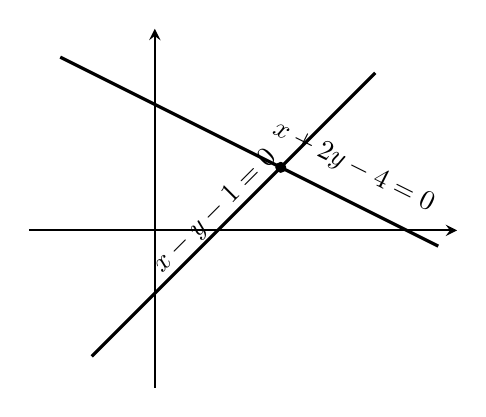
\begin{tikzpicture}[scale=0.8, >=stealth]
  \draw[->, thick] (-2, 0) -- (4.8, 0);
  \draw[->, thick] (0, -2.5) -- (0, 3.2);
  
  % Line 1: x + 2y - 4 = 0
  \draw[very thick] (-1.5, 2.75) -- (4.5, -0.25);
  \node[above, rotate=-26.5] at (3.0, 0.7) {$x+2y-4=0$};
  
  % Line 2: x - y - 1 = 0
  \draw[very thick] (-1, -2) -- (3.5, 2.5);
  \node[above, rotate=45] at (1.2, 0.05) {$x-y-1=0$};
  
  % Intersection (2, 1)
  \fill (2, 1) circle (2.5pt);
\end{tikzpicture}
\caption{相交兩直線}
\label{fig:b4-ch4-fig1-5}
\end{minipage}
\end{figure}

\begin{tcolorbox}[colback=black!5,colframe=black!40,arc=0mm,boxrule=0.5pt,top=1.5mm,bottom=1.5mm,left=2mm,right=2mm]
\textbf{注意：} 視察法在簡單情形下較為迅捷，但並非始終有效．配方法拙而穩當，對任何複雜的情形皆能處理．
\end{tcolorbox}

\begin{example}
$2x^2 - 2xy + y^2 - 6x + 2y + 1 = 0$ 是否特異？若非特異請示其軌跡區域．
\end{example}

\begin{solution}
$\delta = (-1)^2 - 2 \times 1 = -1 < 0$．
\[
\Delta = \begin{vmatrix} 2 & -1 & -3 \\ -1 & 1 & 1 \\ -3 & 1 & 1 \end{vmatrix} = -8 \ne 0.
\]
$H = 2 + 1 = 3 > 0$．因 $\delta < 0, H\Delta = -24 < 0$，故非特異．

又將方程式依 $y$ 之降冪排列整理得：
\[
y^2 - 2(x - 1)y + (2x^2 - 6x + 1) = 0 \tag{$*$}
\]
因為點 $(x, y)$ 在圖形上的充要條件是 $x$ 及 $y$ 要滿足 ($*$)，而由於 $y$ 是實數，我們必須要求判別式大於等於 0：
\[
4(x - 1)^2 - 4(2x^2 - 6x + 1) \ge 0 \implies -x^2 + 4x \ge 0 \implies x(x - 4) \le 0
\]
也就是說 $x$ 要在 $0 \le x \le 4$ 的範圍內．

同理我們若將原式依 $x$ 的降冪排列整理得：
\[
2x^2 - 2(y + 3)x + (y^2 + 2y + 1) = 0
\]
由於 $x$ 是實數，因此 $y$ 必須受 $(y + 3)^2 - 2(y^2 + 2y + 1) \ge 0$ 的限制，亦即 $-y^2 + 2y + 7 \ge 0 \implies y^2 - 2y - 7 \le 0$．解之得：
\[
1 - 2\sqrt{2} \le y \le 1 + 2\sqrt{2}.
\]

\begin{figure}[htbp]
\centering
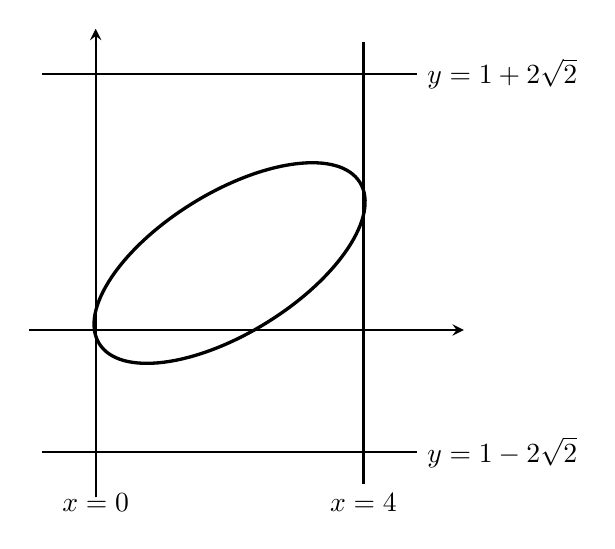
\begin{tikzpicture}[scale=0.85, >=stealth]
  % Axes
  \draw[->, thick] (-1, 0) -- (5.5, 0);
  \draw[->, thick] (0, -2.5) -- (0, 4.5);
  
  % Bounding solid lines matching original
  \draw[thick] (0, -2.3) -- (0, 4.3);
  \node[below] at (0, -2.3) {$x=0$};
  \draw[thick] (4, -2.3) -- (4, 4.3);
  \node[below] at (4, -2.3) {$x=4$};
  \draw[thick] (-0.8, 3.828) -- (4.8, 3.828) node[right] {$y = 1 + 2\sqrt{2}$};
  \draw[thick] (-0.8, -1.828) -- (4.8, -1.828) node[right] {$y = 1 - 2\sqrt{2}$};
  
  % Tilted ellipse tangent to bounding box
  % Center is (2, 1). Matrix: 2x^2 - 2xy + y^2 - 6x + 2y + 1 = 0
  \draw[very thick, rotate around={31.7:(2, 1)}] (2, 1) ellipse (2.29cm and 1.05cm);
\end{tikzpicture}
\caption{橢圓與其外切矩形}
\label{fig:b4-ch4-fig1-6}
\end{figure}

因此圖形應該落在 $0 \le x \le 4, 1 - 2\sqrt{2} \le y \le 1 + 2\sqrt{2}$ 所圍成的長方形內．

事實上這是一個橢圓，它的作圖我們在這一章裏將討論到．
\end{solution}

\begin{tcolorbox}[colback=white,colframe=black!60,arc=0mm,boxrule=0.5pt,top=1.5mm,bottom=1.5mm,left=2mm,right=2mm]
\textbf{〔作業 3〕} $8x^2 + 10xy - 12y^2 - 22x - 11y + 15 = 0$ 是否特異？

\textbf{〔作業 4〕} 試用行列式 $\Delta$ 檢驗方程式 $6x^2 + 13xy - 5y^2 + 9x + 31y - 6 = 0$ 是否代表兩條直線的一次函數的乘積，並作圖求它所描繪兩直線的位置．

\textbf{〔作業 5〕} 在上題中，以 $O'(2, -3)$ 為新原點，平移座標系後，再轉軸 $30^\circ$，求二次曲線的新方程式？它是否仍為二元二次方程式？並求其相應的 $\Delta$．
\end{tcolorbox}

\subsubsection*{習題 IV-1}

依 $\delta, \Delta, H$ 判別下列各式是否特異；若為特異，描繪其軌跡；若非特異，則仿圖 1-1 與圖 1-2 定出其軌跡區域．

\begin{enumerate}
  \item $x^2 + 6xy + y^2 - 10x - 14y + 9 = 0$.
  \item $2x^2 + 4xy - y^2 + 20x + 8y + 32 = 0$.
  \item $4x^2 - 4xy + y^2 + 10x + 6y + 5 = 0$.
  \item $x^2 + 4xy + 4y^2 - 2x - 4y - 3 = 0$.
  \item $2xy - 4x + 2y - 5 = 0$.
  \item $x^2 + 4y^2 - 8x - 16y + 28 = 0$.
  \item $5x^2 + 6xy + 5y^2 = 32$.
  \item $3x^2 + 2\sqrt{3}xy + y^2 + 2x - 2\sqrt{3}y = 0$.
  \item $3x^2 + 4xy + 4 = 0$.
\end{enumerate}


\subsection{§ IV-2\texorpdfstring{\quad }{ }固有值理論}

\subsubsection*{甲、\quad 問題的分析}

先考慮二元二次方程式
\[
Ax^2 + 2Bxy + Cy^2 + 2Dx + 2Ey + F = 0
\]
中的二次項，設之為 $Q(x, y)$，並將 $(x, y)$ 改以 $(x_1, x_2)$ 記述得：
\[
Q(x_1, x_2) \equiv Ax_1^2 + 2Bx_1 x_2 + Cx_2^2.
\]
$Q(x_1, x_2)$ 稱為 $x_1, x_2$ 的一個二次式．

今在平面上考慮自然座標系 $(O; i_1, i_2)$，則 $(x_1, x_2)$ 可視為相應於向量
\[
x = x_1 i_1 + x_2 i_2
\]
之點，而 $Q$ 則可視為 $Q: \mathbb{R}^2 \to \mathbb{R}$ 的一個映射．此因
\[
Q(x) = Ax_1^2 + 2Bx_1 x_2 + Cx_2^2 \in \mathbb{R}.
\]

\begin{figure}[htbp]
\centering
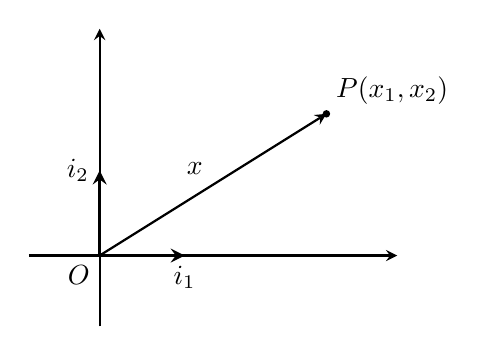
\begin{tikzpicture}[scale=0.9, >=stealth]
  \draw[->, thick] (-1, 0) -- (4.2, 0);
  \draw[->, thick] (0, -1) -- (0, 3.2);
  \node[below left] at (0, 0) {$O$};
  
  % Basis vectors i_1 and i_2
  \draw[->, very thick] (0, 0) -- (1.2, 0) node[below] {$i_1$};
  \draw[->, very thick] (0, 0) -- (0, 1.2) node[left] {$i_2$};
  
  \coordinate (P) at (3.2, 2.0);
  \draw[->, thick] (0, 0) -- (P) node[midway, above left] {$x$};
  \fill (P) circle (1.5pt) node[above right] {$P(x_1, x_2)$};
\end{tikzpicture}
\caption{向量 $x$ 與其自然座標}
\label{fig:b4-ch4-fig2-1}
\end{figure}

但右端其實也可直接以向量 $x$ 來表示，方法如下：

若取一線性映射 $T: \mathbb{R}^2 \to \mathbb{R}^2$ 使得
\[
\begin{cases}
Ti_1 = Ai_1 + Bi_2 \\
Ti_2 = Bi_1 + Ci_2
\end{cases}
\]
亦即 $T$ 的自然矩陣表示為
\[
[T] = \begin{pmatrix} A & B \\ B & C \end{pmatrix}
\]
則
\[
\begin{aligned}
Tx &= T(x_1 i_1 + x_2 i_2) = x_1 Ti_1 + x_2 Ti_2 \\
&= (Ax_1 + Bx_2)i_1 + (Bx_1 + Cx_2)i_2
\end{aligned}
\]
因此 $Tx$ 與 $x$ 的內積為：
\[
\begin{aligned}
Tx \cdot x &= (Ax_1 + Bx_2)x_1 + (Bx_1 + Cx_2)x_2 \\
&= Ax_1^2 + 2Bx_1 x_2 + Cx_2^2\phantomsection\label{note:b4-ch4-tx-image}\footnote{【原書註記】：$Ti_1, Ti_2, Tx$ 等意指 $i_1, i_2, x$ 在映射 $T$ 之下的像．}
\end{aligned}
\]
亦即
\begin{equation}
Q(x) = Tx \cdot x
\label{eq:b4-ch4-quadratic-form-inner-prod}
\end{equation}
（這個式子是二次式理論的一個關鍵，如此 $Q$ 的討論可歸之於線性映射 $T$ 的討論！）

我們現時的目的是要找一個新正交座標系 $(O; e_1, e_2)$ 使得 $x$ 表為 $x_1' e_1 + x_2' e_2$ 時，$Q(x)$ 中不含 $x_1' x_2'$ 項，亦即
\begin{equation}
Q(x) = \lambda_1 {x_1'}^2 + \lambda_2 {x_2'}^2
\label{eq:b4-ch4-diagonalized-form}
\end{equation}
這樣的過程，我們稱為二次式 $Q$ 的\textbf{標準化}．

如果我們能取得一正交基底 $\{e_1, e_2\}$，使得
\begin{equation}
\begin{cases}
Te_1 = \lambda_1 e_1 \\
Te_2 = \lambda_2 e_2
\end{cases}
\label{eq:b4-ch4-eigen-decomp}
\end{equation}
成立，則
\begin{equation}
Tx \cdot x = (\lambda_1 x_1' e_1 + \lambda_2 x_2' e_2) \cdot (x_1' e_1 + x_2' e_2) = \lambda_1 {x_1'}^2 + \lambda_2 {x_2'}^2
\label{eq:b4-ch4-diagonalized-inner-prod}
\end{equation}
我們二次式的標準化便告完成，而所剩的問題便是如何求得滿足 \eqref{eq:b4-ch4-eigen-decomp} 式的 $\lambda_i$ 與 $e_i$，而這一問題便劃入\textbf{固有值的理論}範圍．

\subsubsection*{乙、\quad 固有值與固有向量的求法}

\begin{definition}
設 $T: \mathbb{R}^2 \to \mathbb{R}^2$ 為一線性映射．對一個實數 $\lambda$，若可找到一個向量 $v \ne 0$，使得
\begin{equation}
Tv = \lambda v
\label{eq:b4-ch4-eigen-def}
\end{equation}
則 $\lambda$ 稱為 $T$ 的一個\textbf{固有值}，$v$ 稱為對應於 $\lambda$ 的 $T$ 的一個\textbf{固有向量}．
\end{definition}

直觀地來看：一個非零向量若經 $T$ 映射後方向不變或與原來方向正好相反（但長度可能伸縮），則這向量為一固有向量．注意，並不是每一個線性映射都有固有向量，例如是以 $O$ 為心，將平面旋轉 $\theta$ 角的一個線性映射，若 $0 < \theta < \pi$ 或 $\pi < \theta < 2\pi$，則所有向量經 $T$ 映射後，方向都已改變且不變成與原來方向相反的方向，故 $T$ 無固有向量（當 $\theta = 0, \pi,$ 或 $2\pi$ 時有兩個線性無關的固有向量，其相應固有值為何？）．

\begin{figure}[htbp]
\centering
\begin{minipage}{0.48\textwidth}
\centering
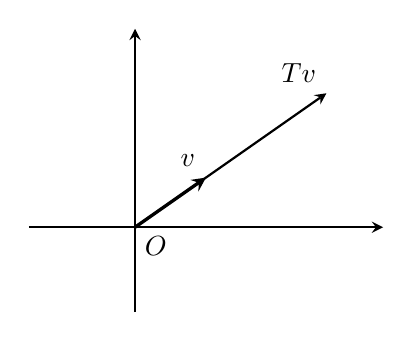
\begin{tikzpicture}[scale=0.9, >=stealth]
  \draw[->, thick] (-1.5, 0) -- (3.5, 0);
  \draw[->, thick] (0, -1.2) -- (0, 2.8);
  \node[below right] at (0, 0) {$O$};
  
  \coordinate (V) at (1.0, 0.7);
  \coordinate (TV) at (2.7, 1.89);
  
  \draw[->, thick] (0, 0) -- (TV) node[above left] {$Tv$};
  \draw[->, very thick] (0, 0) -- (V) node[above left] {$v$};
\end{tikzpicture}
\\[4pt]
\small （此圖 $Tv = 2.7v$，$v$ 為固有向量，\\ \small $2.7$ 為其相應固有值）
\end{minipage}
\hfill
\begin{minipage}{0.48\textwidth}
\centering
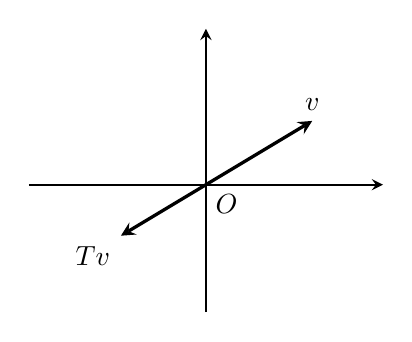
\begin{tikzpicture}[scale=0.9, >=stealth]
  \draw[->, thick] (-2.5, 0) -- (2.5, 0);
  \draw[->, thick] (0, -1.8) -- (0, 2.2);
  \node[below right] at (0, 0) {$O$};
  
  \coordinate (V) at (1.5, 0.9);
  \coordinate (TV) at (-1.2, -0.72);
  
  \draw[->, very thick] (0, 0) -- (V) node[above] {$v$};
  \draw[->, very thick] (0, 0) -- (TV) node[below left] {$Tv$};
\end{tikzpicture}
\\[4pt]
\small （此圖 $Tv = -0.8v$，$v$ 為固有向量，\\ \small $-0.8$ 為相應固有值）
\end{minipage}
\caption{固有向量與固有值的幾何意義}
\label{fig:b4-ch4-fig2-2}
\end{figure}

根據上述固有值與固有向量的定義，我們要找滿足 \eqref{eq:b4-ch4-eigen-decomp} 式的 $e_1, e_2$，就是要找一對相互正交的固有向量 $e_1, e_2$ 及其相應的固有值 $\lambda_1, \lambda_2$．

要在 \eqref{eq:b4-ch4-eigen-def} 式 $Tv = \lambda v$ 中同時解得 $\lambda$ 與 $v$ 兩樣未知物，通常是一件困難的事．我們的方法是將 \eqref{eq:b4-ch4-eigen-def} 式轉化成一個只牽涉 $\lambda$ 的方程式（稱為 $T$ 的\textbf{特徵方程式}）．

\eqref{eq:b4-ch4-eigen-def} 式的意義其實是對 $\lambda$，存在 $v \ne 0$ 使得
\begin{equation}
(T - \lambda I)v = 0
\label{eq:b4-ch4-eigen-null-space}
\end{equation}
式中把 $T - \lambda I$ 看成是一個 $\mathbb{R}^2 \to \mathbb{R}^2$ 的線性映射，其定義為 $(T - \lambda I)(x) = Tx - \lambda x$．於是 \eqref{eq:b4-ch4-eigen-null-space} 式的條件其實就是「$T - \lambda I$ 這一線性映射不是單射」的意思，由第一章知其充要條件為
\begin{equation}
\det[T - \lambda I] = 0
\label{eq:b4-ch4-char-poly-det}
\end{equation}
其中 $[T - \lambda I]$ 表 $T - \lambda I$ 之自然矩陣表示，這 \eqref{eq:b4-ch4-char-poly-det} 式稱為 $T$ 相關於自然座標系之\textbf{特徵方程式}（或稱自然特徵方程式）．

但注意如果 $T$ 的自然矩陣表示為 $[T] = \begin{pmatrix} a_{11} & a_{12} \\ a_{21} & a_{22} \end{pmatrix}$，則 $T - \lambda I$ 的矩陣表示（對同一座標系）為
\[
[T - \lambda I] = \begin{pmatrix} a_{11} - \lambda & a_{12} \\ a_{21} & a_{22} - \lambda \end{pmatrix} \quad \text{〔請讀者驗證〕}
\]
故 \eqref{eq:b4-ch4-char-poly-det} 式化成 $\lambda$ 的一個一元二次方程式：
\begin{equation}
\lambda^2 - (a_{11} + a_{22})\lambda + \begin{vmatrix} a_{11} & a_{12} \\ a_{21} & a_{22} \end{vmatrix} = 0
\label{eq:b4-ch4-char-poly-expanded}
\end{equation}
這便是 $T$ 的自然特徵方程式的另一形式．當 $a_{12} = a_{21}$ 時我們稱 $[T]$ 為\textbf{對稱矩陣}，此時特徵方程式中的 $\lambda$ 一定有實數解，此因其判別式：
\[
\begin{aligned}
(a_{11} + a_{22})^2 - 4\begin{vmatrix} a_{11} & a_{12} \\ a_{21} & a_{22} \end{vmatrix}
&= (a_{11}^2 - 2a_{11} a_{22} + a_{22}^2) + 4a_{12} a_{21} \\
&= (a_{11} - a_{22})^2 + 4a_{12}^2 \ge 0.
\end{aligned}
\]
這（些）解便是 $T$ 的固有值〔一般時候 \eqref{eq:b4-ch4-char-poly-expanded} 式也可能無解，此時無固有值（作業 6）〕．

而當求得固有值之後，便可將其代入 \eqref{eq:b4-ch4-eigen-null-space} 式中解得固有向量．詳細解法如下：

設 $v$ 之自然座標為 $(x_1, x_2)$，則因
\[
Tv = x_1 (a_{11} i_1 + a_{21} i_2) + x_2 (a_{12} i_1 + a_{22} i_2) = [(a_{11} - \lambda)x_1 + a_{12} x_2]i_1 + [a_{21} x_1 + (a_{22} - \lambda)x_2]i_2,
\]
故解 $(T - \lambda I)v = 0$ 相當於解下列聯立方程式：
\begin{equation}
\begin{cases}
(a_{11} - \lambda)x_1 + a_{12} x_2 = 0 \\
a_{21} x_1 + (a_{22} - \lambda)x_2 = 0
\end{cases}
\label{eq:b4-ch4-eigen-system}
\end{equation}
中的 $x_1, x_2$．

\begin{tcolorbox}[colback=white,colframe=black!60,arc=0mm,boxrule=0.5pt,top=1.5mm,bottom=1.5mm,left=2mm,right=2mm]
\textbf{〔作業 6〕} 當 $T$ 為旋轉 $\begin{pmatrix} \cos\theta & -\sin\theta \\ \sin\theta & \cos\theta \end{pmatrix}$ 時，$\theta \ne n\pi, n \in \mathbb{Z}$，試證 $T$ 無固有值．

\textbf{〔作業 7〕} 求鏡射 $\begin{pmatrix} 1 & 0 \\ 0 & -1 \end{pmatrix}$ 的固有值．
\end{tcolorbox}

\begin{example-non}
【論例 1】 設 $[T] = \begin{pmatrix} 3 & 2 \\ 2 & 6 \end{pmatrix}$ 為 $T$ 的自然矩陣表示，亦即 $Ti_1 = 3i_1 + 2i_2, Ti_2 = 2i_1 + 6i_2$．找其固有值、固有向量及單位長的固有向量．
\end{example-non}

\begin{solution}
\begin{enumerate}[(i)]
  \item 若解特徵方程式
  \[
  \begin{vmatrix} 3 - \lambda & 2 \\ 2 & 6 - \lambda \end{vmatrix} = 0
  \]
  中之 $\lambda$ 即得 $T$ 之固有值如下：將上式化成
  \[
  \lambda^2 - 9\lambda + (18 - 4) = 0 \iff (\lambda - 2)(\lambda - 7) = 0.
  \]
  故得兩固有值：$\lambda_1 = 2, \lambda_2 = 7$．

  \item 欲求其相應的固有向量．設 $\lambda$ 已知為 2，從 $(T - 2I)v = 0$ 中解出 $v$，此相當於要從
  \[
  \begin{cases}
  (3 - 2)x_1 + 2x_2 = 0 \\
  2x_1 + (6 - 2)x_2 = 0
  \end{cases}
  \iff
  \begin{cases}
  x_1 + 2x_2 = 0 \\
  2x_1 + 4x_2 = 0
  \end{cases}
  \]
  中解出 $x_1, x_2$．此表示兩式為相依方程式，有無限多解，而 $x_1$ 與 $x_2$ 的關係為：
  \[
  x_1 = -2x_2.
  \]
  換句話說，取 $x_2 = t$，則任意自然座標可表為 $(-2t, t)$ 之向量 $v$ 皆為解，亦即
  \[
  v = (-2t, t)
  \]
  為相應於 $\lambda = 2$ 之固有向量，式中 $t$ 為任意非零實數．

  \item 若要求出一單位長的固有向量，則 $t$ 須滿足 $\sqrt{(-2t)^2 + t^2} = 1 \implies \sqrt{5}|t| = 1 \implies t = \pm \dfrac{1}{\sqrt{5}}$．即
  \[
  e_1 = \left( -\frac{2}{\sqrt{5}}, \frac{1}{\sqrt{5}} \right) \quad \text{或} \quad \left( \frac{2}{\sqrt{5}}, -\frac{1}{\sqrt{5}} \right).
  \]
  至於 $\lambda = 7$ 所相應之固有向量 $v'$，同法可解得〔留當作業〕：
  \[
  v' = (t, 2t), \quad t \text{ 為任意實數}
  \]
  若取為單位長，則必有
  \[
  e_2 = \left( \frac{1}{\sqrt{5}}, \frac{2}{\sqrt{5}} \right) \quad \text{或} \quad \left( -\frac{1}{\sqrt{5}}, -\frac{2}{\sqrt{5}} \right).
  \]
\end{enumerate}
\end{solution}

\begin{tcolorbox}[colback=black!5,colframe=black!40,arc=0mm,boxrule=0.5pt,top=1.5mm,bottom=1.5mm,left=2mm,right=2mm]
\textbf{注意：} 在本論例中 $v$ 與 $v'$ 垂直，此因 $v \cdot v' = (-2t)(t') + (t)(2t') = 0$．這一現象並非巧合，我們將證得：
\end{tcolorbox}

\begin{proposition}
設一線性映射 $T$ 的自然矩陣表示 $[T] = \begin{pmatrix} a_{11} & a_{12} \\ a_{21} & a_{22} \end{pmatrix}$ 中，$a_{12} = a_{21}$〔此時稱 $[T]$ 為對稱〕．若 $v, v'$ 為相應於 $T$ 的兩個固有值 $\lambda_1, \lambda_2$ 的固有向量，且 $\lambda_1 \ne \lambda_2$，則 $v$ 與 $v'$ 相互垂直，亦即
\[
v \cdot v' = 0.
\]
\end{proposition}

\begin{proof}
由假設 $Tv = \lambda_1 v$ 及 $Tv' = \lambda_2 v'$，兩端分別取內積：
\[
(Tv) \cdot v' = (\lambda_1 v) \cdot v' = \lambda_1 (v \cdot v'), \qquad
v \cdot (Tv') = v \cdot (\lambda_2 v') = \lambda_2 (v \cdot v').
\]
而兩式左端以座標表示展開，分別為：
\[
\begin{aligned}
(Tv) \cdot v' &= a_{11} x_1 x_1' + a_{21} x_2 x_1' + a_{12} x_1 x_2' + a_{22} x_2 x_2', \\
v \cdot (Tv') &= a_{11} x_1 x_1' + a_{12} x_2 x_1' + a_{21} x_1 x_2' + a_{22} x_2 x_2'.
\end{aligned}
\]
但 $a_{12} = a_{21}$，故 $(Tv) \cdot v' = v \cdot (Tv')$，即
\[
\lambda_1 (v \cdot v') = \lambda_2 (v \cdot v') \implies (\lambda_1 - \lambda_2)(v \cdot v') = 0.
\]
而 $\lambda_1 \ne \lambda_2$，故
\[
v \cdot v' = 0.
\]
\end{proof}

這命題使我們以後若知有兩線性無關，且相應於不同固有值的固有向量，則只須找出其一（比如說 $v$）而取 $v'$ 為一垂直於 $v$ 的向量，則 $v'$ 必亦為固有向量．〔這事在下節論例 3，4 中將被採用〕

\begin{tcolorbox}[colback=white,colframe=black!60,arc=0mm,boxrule=0.5pt,top=1.5mm,bottom=1.5mm,left=2mm,right=2mm]
\textbf{〔作業 8〕}
\begin{enumerate}[(i)]
  \item 試完成論例 1．
  \item 設 $[T] = \begin{pmatrix} 17 & 6 \\ 6 & 8 \end{pmatrix}$ 為 $T$ 的自然矩陣表示．試求其固有值，固有向量及單位長的固有向量．
\end{enumerate}
\end{tcolorbox}

\subsubsection*{習題 IV-2}

下列各矩陣都是自然矩陣表示，試問它們有無固有值？若有則求固有值，固有向量及單位長度固有向量．

\begin{enumerate}
  \item $\begin{pmatrix} 1 & 1 \\ 1 & 1 \end{pmatrix}$.
  \item $\begin{pmatrix} 1 & 0 \\ 0 & k \end{pmatrix}, \quad k \ne 0$.
  \item $\begin{pmatrix} 5 & 3 \\ 3 & 2 \end{pmatrix}$.
  \item $\begin{pmatrix} 6 & 2 \\ 2 & 3 \end{pmatrix}$.
  \item $\begin{pmatrix} 1 & 2 \\ -\frac{1}{2} & \frac{1}{2} \end{pmatrix}$.
  \item $\begin{pmatrix} 3 & 1 \\ 2 & 2 \end{pmatrix}$.
\end{enumerate}


\subsection{§ IV-3\texorpdfstring{\quad }{ }二次式的標準化}

上節的固有值理論已經告訴我們如何依循甲段中的分析實際求算 \eqref{eq:b4-ch4-eigen-decomp} 式中的 $\lambda_i$ 及 $e_i$，上節命題 4 使我們在取 $e_1, e_2$ 為兩個單位長的固有向量時，可以要求 $e_1$ 與 $e_2$ 垂直，即
\[
e_1 \cdot e_2 = 0.
\]
因此我們可取新正交座標系 $(O; e_1, e_2)$ 將 $Q(x)$ 標準化．

因為 $\{e_1, e_2\}, \{i_1, i_2\}$ 皆為正交基底，故由第一章剛性運動的分類知這兩基底間的關係只有兩種：
\begin{enumerate}[(i)]
  \item \textbf{旋轉：} 此時 $e_1, e_2$ 可表成
  \begin{equation}
  \begin{cases}
  e_1 = \cos\theta i_1 + \sin\theta i_2 \\
  e_2 = -\sin\theta i_1 + \cos\theta i_2
  \end{cases}
  \label{eq:b4-ch4-rot-basis}
  \end{equation}
  \item \textbf{鏡射：} 此時 $e_1, e_2$ 可表成
  \begin{equation}
  \begin{cases}
  e_1 = \cos\theta i_1 + \sin\theta i_2 \\
  e_2 = \sin\theta i_1 - \cos\theta i_2
  \end{cases}
  \label{eq:b4-ch4-refl-basis}
  \end{equation}
\end{enumerate}

\begin{definition}
二次式 $Q(x_1, x_2)$ 標準化
\[
Q(x_1, x_2) = \lambda_1 {x_1'}^2 + \lambda_2 {x_2'}^2
\]
後所採用的新基底 $\{e_1, e_2\}$，若自舊基底 $\{i_1, i_2\}$ 旋轉角度 $\theta$ 而得，則稱這新基底為\textbf{正性基底}，而這標準化的過程為\textbf{正性標準化}．此時：
\begin{equation}
\begin{cases}
x_1 = \cos\theta x_1' - \sin\theta x_2' \\
x_2 = \sin\theta x_1' + \cos\theta x_2'
\end{cases}
\label{eq:b4-ch4-pos-standard-coord}
\end{equation}
另一種可能是由鏡射而得，此時稱這新基底為\textbf{負性基底}，而稱相應標準化的過程為\textbf{負性標準化}．而知
\begin{equation}
\begin{cases}
x_1 = \cos\theta x_1' + \sin\theta x_2' \\
x_2 = \sin\theta x_1' - \cos\theta x_2'
\end{cases}
\label{eq:b4-ch4-neg-standard-coord}
\end{equation}
\end{definition}

基於以上二次式標準化的討論，二次式經正性與負性標準化的結果並無差異，同樣都是 $\lambda_1 {x_1'}^2 + \lambda_2 {x_2'}^2$，因為 $e_1, e_2$ 不論取成 \eqref{eq:b4-ch4-rot-basis} 式或 \eqref{eq:b4-ch4-refl-basis} 式，它們皆仍分別為固有值為 $\lambda_1, \lambda_2$ 的 $T$ 的固有向量．

\begin{example-non}
【論例 2】 將二次式 $3x^2 + 4xy + 6y^2$ 標準化，並求標準化中新舊座標間的關係．
\end{example-non}

\begin{solution}
設 $Q(x) = 3x_1^2 + 4x_1 x_2 + 6x_2^2$，其中 $x = (x_1, x_2)$ 為自然座標．取 $T: \mathbb{R}^2 \to \mathbb{R}^2$，其自然矩陣表示為
\[
[T] = \begin{pmatrix} 3 & 2 \\ 2 & 6 \end{pmatrix}
\]
則 $Q(x) = Tx \cdot x$．而論例 1 中已證得 $T$ 之兩個固有值為
\[
\lambda_1 = 2, \quad \lambda_2 = 7
\]
而兩單位固有向量 $e_1, e_2$ 可取為
\[
e_1 = \left( -\frac{2}{\sqrt{5}}, \frac{1}{\sqrt{5}} \right), \qquad
e_2 = \left( -\frac{1}{\sqrt{5}}, -\frac{2}{\sqrt{5}} \right)
\]
〔此為正性標準化，若取 $e_2 = \left( \frac{1}{\sqrt{5}}, \frac{2}{\sqrt{5}} \right)$ 則為負性；$Q$ 標準化後仍是 $2{x_1'}^2 + 7{x_2'}^2$〕．故據 § IV-2 中 \eqref{eq:b4-ch4-diagonalized-inner-prod} 式得
\[
Q(x) = 2{x_1'}^2 + 7{x_2'}^2
\]
其中 $(x_1', x_2')$ 為 $x$ 相關於 $(O; e_1, e_2)$ 的座標，其與舊座標的關係為：
\[
\begin{cases}
x_1 = -\dfrac{2}{\sqrt{5}}x_1' - \dfrac{1}{\sqrt{5}}x_2' \\[0.5em]
x_2 = \dfrac{1}{\sqrt{5}}x_1' - \dfrac{2}{\sqrt{5}}x_2'
\end{cases}
\]
故 $3x^2 + 4xy + 6y^2$ 標準化後成 $2{x'}^2 + 7{y'}^2$．有時不再強調 $('$ 之異於 $(x, y)$，而逕記上式為 $2x^2 + 7y^2$．
\end{solution}

\begin{tcolorbox}[colback=black!5,colframe=black!40,arc=0mm,boxrule=0.5pt,top=1.5mm,bottom=1.5mm,left=2mm,right=2mm]
\textbf{注意：} 本論例中 $\delta = B^2 - AC = 4 - 18 = -14 < 0$；$H = 3 + 6 = 9$．標準化後仍然 $\delta = 0 - 2 \times 7 = -14 < 0$；$H = 2 + 7 = 9$．
\end{tcolorbox}

我們總結一下本節的討論：

若 $Q(x, y) = Ax^2 + 2Bxy + Cy^2$，$B \ne 0$\phantomsection\label{note:b4-ch4-b-zero}\footnote{【原書註記】：$B = 0$ 時，就不須再化簡了．}，且 $(x, y)$ 表示平面上點的自然座標，我們可找到一個正交座標系 $(O; e_1, e_2)$，其中
\[
\begin{cases}
e_1 = \cos\theta i_1 + \sin\theta i_2 \\
e_2 = -\sin\theta i_1 + \cos\theta i_2
\end{cases}
\quad \text{〔代表座標系的一旋轉〕}
\]
使 $Q(x, y)$ 化成如下較簡的形式：
\begin{center}
\textbf{化簡的方法：}
\end{center}
\begin{enumerate}[(i)]
  \item 取 $[T] = \begin{pmatrix} A & B \\ B & C \end{pmatrix}$（$B \ne 0$），而自特徵方程式
  \[
  \begin{vmatrix} A - \lambda & B \\ B & C - \lambda \end{vmatrix} = 0
  \]
  中解出 $\lambda$，此特徵方程式必有相異兩實根 $\lambda_1, \lambda_2$．
  
  \item 從下式
  \[
  (T - \lambda_1 I)x = 0 \iff
  \begin{cases}
  (A - \lambda_1)x_1 + Bx_2 = 0 \\
  Bx_1 + (C - \lambda_1)x_2 = 0
  \end{cases}
  \]
  解出一個單位固有向量 $e_1$，可表為
  \[
  e_1 = (\cos\theta, \sin\theta) = \cos\theta i_1 + \sin\theta i_2.
  \]
  
  \item 然後取\phantomsection\label{note:b4-ch4-e2-choice}\footnote{【原書註記】：若取 $e_2 = (\sin\theta, -\cos\theta) = \sin\theta i_1 - \cos\theta i_2$，則使 $Q$ 負性標準化．}
  \[
  e_2 = (-\sin\theta, \cos\theta) = -\sin\theta i_1 + \cos\theta i_2
  \]
  其中 $\theta$ 的幾何意義是 $\theta$ 為舊座標系 $(O; i_1, i_2)$ 到新座標系 $(O; e_1, e_2)$ 的轉角角度．則 $e_1, e_2$ 滿足 $Te_1 = \lambda_1 e_1, Te_2 = \lambda_2 e_2$，而得新舊座標之關係如下：
  \[
  \begin{cases}
  x_1 = \cos\theta x_1' - \sin\theta x_2' \\
  x_2 = \sin\theta x_1' + \cos\theta x_2'
  \end{cases}
  \]
  這使 $Q(x_1, x_2)$ 得以正性標準化．
\end{enumerate}

\begin{figure}[htbp]
\centering
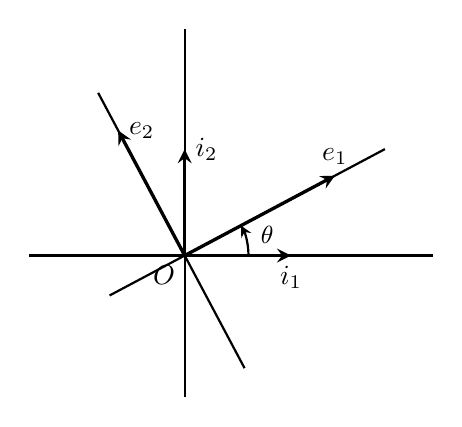
\begin{tikzpicture}[scale=0.9, >=stealth]
  % Old axes: horizontal and vertical
  \draw[thick] (-2.2, 0) -- (3.5, 0);
  \draw[->, very thick] (0, 0) -- (1.5, 0) node[below] {$i_1$};
  \draw[thick] (0, -2.0) -- (0, 3.2);
  \draw[->, very thick] (0, 0) -- (0, 1.5) node[right] {$i_2$};
  \node[below left] at (0, 0) {$O$};
  
  % Rotated new axes: e_1 and e_2
  \def\ang{28}
  % Axis for e_1 line
  \draw[thick] ({\ang+180}:1.2) -- ({\ang}:3.2);
  \draw[->, very thick] (0, 0) -- ({\ang}:2.4) node[above] {$e_1$};
  
  % Axis for e_2 line (perpendicular to e_1)
  \draw[thick] ({\ang+270}:1.8) -- ({\ang+90}:2.6);
  \draw[->, very thick] (0, 0) -- ({\ang+90}:2.0) node[right] {$e_2$};
  
  % Angle arc theta between i_1 and e_1
  \draw[->, thick] (0.9, 0) arc (0:\ang:0.9);
  \node at (14:1.2) {\small $\theta$};
\end{tikzpicture}
\caption{轉角 $\theta$ 與新正交基底}
\label{fig:b4-ch4-fig3-1}
\end{figure}

\begin{example-non}
【論例 3】 將二次式 $x^2 + 2xy + y^2$ 標準化，並求標準化中新舊座標間之關係．
\end{example-non}

\begin{solution}
\begin{enumerate}[(i)]
  \item 特徵方程式為
  \[
  \begin{vmatrix} 1 - \lambda & 1 \\ 1 & 1 - \lambda \end{vmatrix} = 0 \iff (1 - \lambda)^2 - 1 = 0 \iff \lambda(\lambda - 2) = 0.
  \]
  故兩固有值為 $\lambda_1 = 2, \lambda_2 = 0$．根據上述理論 $Q(x, y)$ 化成 $2{x'}^2$．
  
  \item 欲求新舊座標間的關係則須確知所取的 $e_1$ 與 $e_2$，亦即須解
  \[
  \begin{cases}
  (1 - \lambda)x_1 + x_2 = 0 \\
  x_1 + (1 - \lambda)x_2 = 0
  \end{cases}
  \]
  當 $\lambda = 2$，得 $-x_1 + x_2 = 0 \implies x_1 = x_2$．單位長度解為
  \[
  e_1 = \left( \frac{1}{\sqrt{2}}, \frac{1}{\sqrt{2}} \right).
  \]
  因 $e_2 \cdot e_1 = 0$，故 $e_2$ 為相應於另一固有值 $\lambda = 0$ 之單位固有向量：
  \[
  e_2 = \left( -\frac{1}{\sqrt{2}}, \frac{1}{\sqrt{2}} \right).
  \]
  其與舊座標之關係為：
  \[
  \begin{cases}
  x = \dfrac{1}{\sqrt{2}}x' - \dfrac{1}{\sqrt{2}}y' \\[0.5em]
  y = \dfrac{1}{\sqrt{2}}x' + \dfrac{1}{\sqrt{2}}y'
  \end{cases}
  \]
  則二次式為 $2{x'}^2$．
\end{enumerate}
\end{solution}

\begin{tcolorbox}[colback=black!5,colframe=black!40,arc=0mm,boxrule=0.5pt,top=1.5mm,bottom=1.5mm,left=2mm,right=2mm]
\textbf{注意：} 本論例 3 中 $\delta = B^2 - AC = 1 - 1 = 0$；$H = 1 + 1 = 2$．標準化後仍為 $\delta = 0 - 2 \times 0 = 0$；$H = 2 + 0 = 2$．
\end{tcolorbox}

\begin{example-non}
【論例 4】 將二次式 $3x^2 + 8xy + 3y^2$ 標準化，並求標準化中新舊座標間的關係．
\end{example-non}

\begin{solution}
\begin{enumerate}[(i)]
  \item 使其自然矩陣表示為 $[T] = \begin{pmatrix} 3 & 4 \\ 4 & 3 \end{pmatrix}$，而特徵方程式：
  \[
  \begin{vmatrix} 3 - \lambda & 4 \\ 4 & 3 - \lambda \end{vmatrix} = 0 \iff (3 - \lambda)^2 - 16 = 0 \iff \lambda^2 - 6\lambda - 7 = 0 \iff (\lambda + 1)(\lambda - 7) = 0.
  \]
  故有二固有值為 $\lambda_1 = -1, \lambda_2 = 7$．根據上述理論 $Q(x)$ 可化成 $-{x'}^2 + 7{y'}^2$．
  
  \item 欲求 $e_1, e_2$，可解：
  \[
  \begin{cases}
  (3 - \lambda)x + 4y = 0 \\
  4x + (3 - \lambda)y = 0
  \end{cases}
  \]
  取 $\lambda = -1$，得 $4x + 4y = 0 \implies x = -y$．取長度為 1 者：
  \[
  e_1 = \left( \frac{1}{\sqrt{2}}, -\frac{1}{\sqrt{2}} \right).
  \]
  則根據命題 4 取垂直向量：
  \[
  e_2 = \left( \frac{1}{\sqrt{2}}, \frac{1}{\sqrt{2}} \right)
  \]
  亦為一固有向量（相應於固有值 $\lambda_2 = 7$）．其新舊座標變換式應為：
  \[
  \begin{cases}
  x = \dfrac{1}{\sqrt{2}}x' + \dfrac{1}{\sqrt{2}}y' \\[0.5em]
  y = -\dfrac{1}{\sqrt{2}}x' + \dfrac{1}{\sqrt{2}}y'
  \end{cases}
  \]
  且有 $Q = -{x'}^2 + 7{y'}^2$．
\end{enumerate}
\end{solution}

\begin{tcolorbox}[colback=black!5,colframe=black!40,arc=0mm,boxrule=0.5pt,top=1.5mm,bottom=1.5mm,left=2mm,right=2mm]
\textbf{注意：} 本論例中二次式 $Q(x) = 3x^2 + 8xy + 3y^2$ 標準化成 $-{x'}^2 + 7{y'}^2$ 後，$B^2 - AC$ 值不變．此因 $4^2 - 9 = 7$；$0 - (-1)(7) = 7$．
\end{tcolorbox}

在以上三論例中我們注意到 $\delta$ 與 $H$ 的值不因標準化而變，事實上這一現象亦非巧合，我們將證得：

\begin{theorem}[不變量定理]
設二次式根據兩個同原點的正交座標系 $S = (O; e_1, e_2)$ 與 $\bar{S} = (O; \bar{e}_1, \bar{e}_2)$ 之表示分別為
\begin{align}
Q(x) &= Ax^2 + 2Bxy + Cy^2 \label{eq:b4-ch4-thm2-q1} \\
\bar{Q}(\bar{x}) &= \bar{A}\bar{x}^2 + 2\bar{B}\bar{x}\bar{y} + \bar{C}\bar{y}^2 \label{eq:b4-ch4-thm2-q2}
\end{align}
則
\begin{equation}
\begin{aligned}
B^2 - AC &= \bar{B}^2 - \bar{A}\bar{C} \\
A + C &= \bar{A} + \bar{C}
\end{aligned}
\label{eq:b4-ch4-thm2-invariants}
\end{equation}
亦即令 $B^2 - AC = -\text{行列式} \begin{vmatrix} A & B \\ B & C \end{vmatrix}$，$A + C =$ 矩陣 $\begin{pmatrix} A & B \\ B & C \end{pmatrix}$ 對角線上元素的和（稱為此矩陣的跡），則 $\delta$ 與 $H$ 是旋轉或鏡射變換下的不變量．
\end{theorem}

\begin{proof}
$Q(x)$ 可表為 $Q(x) = Tx \cdot x$．考慮可找到 $x \ne 0$ 使 $Tx = \lambda x$ 的實數 $\lambda$，這樣的 $\lambda$ 與 $x$ 的座標選取無關（道理是 $T$ 因 $Q$ 而決定，而 $Q$ 的定義並不依賴於座標）．

而這樣的 $\lambda$ 不管 $T$ 的矩陣表示相關於那一座標系，即不管取 $[T]_S$ 或 $[T]_{\bar{S}}$，皆有
\[
\det[T - \lambda I]_S = 0 \iff \lambda^2 - (A + C)\lambda - (B^2 - AC) = 0,
\]
\[
\det[T - \lambda I]_{\bar{S}} = 0 \iff \lambda^2 - (\bar{A} + \bar{C})\lambda - (\bar{B}^2 - \bar{A}\bar{C}) = 0.
\]
兩個方程式的根均為 $T$ 的固有值，設 $\lambda_1, \lambda_2$ 為兩方程式的兩個共同根，由根與係數的關係：
\[
A + C = \lambda_1 + \lambda_2 = \bar{A} + \bar{C},
\]
\[
-(B^2 - AC) = \lambda_1 \lambda_2 = -(\bar{B}^2 - \bar{A}\bar{C}) \implies B^2 - AC = \bar{B}^2 - \bar{A}\bar{C}.
\]
\end{proof}

\subsubsection*{習題 IV-3}

\textbf{一、} 試將下列二次式標準化，並求標準化中新舊座標間的關係：
\begin{enumerate}
  \item $3x^2 + 2\sqrt{3}xy + y^2$.
  \item $4x^2 - 4xy + y^2$.
  \item $2xy$.
  \item $25x^2 + 14xy + 25y^2$.
  \item $95x^2 + 54xy - 10y^2$.
\end{enumerate}

\textbf{二、} 試將下列二次曲線的二次項式標準化，能否利用標準化中新舊座標間的關係及配方法將二次曲線的方程式化成只有二次項及常數項的形式？
\begin{enumerate}
  \item $x^2 + 4xy + y^2 = 16$.
  \item $x^2 + 6xy + y^2 - 10x - 14y + 9 = 0$.
  \item $3x^2 - 4xy + 8x - 1 = 0$.
  \item $14x^2 - 4xy + 11y^2 - 88x + 34y + 149 = 0$.
\end{enumerate}
可否從所化得形式看出二次曲線的類別？


\subsection{§ IV-4\texorpdfstring{\quad }{ }不變量}

\subsubsection*{甲、\quad 空間的二次幾何}

在進入二次曲線的分類定理之前，我們討論一下空間的二次幾何：

對於一個二元函數
\begin{equation}
z = f(x, y); \quad (x, y) \in \Omega \subset \mathbb{R}^2
\label{eq:b4-ch4-surface-func}
\end{equation}
其中 $f: \Omega \to \mathbb{R}$，$(x, y)$ 為 $\Omega$ 上點的自然座標．我們常仿照一元函數在平面上以其函數曲線描述的辦法繪一曲面來描述 $f$：對任意 $(x, y) \in \Omega \subset \mathbb{R}^2$，取空間 $\mathbb{R}^3$ 中的點 $(x, y, z)$，使
\[
z = f(x, y)
\]
亦即取
\[
S = \{ (x, y, z) \in \mathbb{R}^3 \mid z = f(x, y), (x, y) \in \Omega \},
\]
則 $S$ 呈一曲面形狀，$S$ 稱為 $f(x, y)$ 的\textbf{函數圖形}．

如果我們把 $f(x, y)$ 視為在 $(x, y)$ 點上的溫度，常常我們要了解其函數圖形的方法是在 $XY$-平面上畫 $f(x, y)$ 之值為定常的一系列曲線：
\begin{equation}
f(x, y) = c; \quad c \text{ 為常數}
\label{eq:b4-ch4-level-curves}
\end{equation}
換句話說，對每一實數 $c$，考慮溫度為 $c$ 度的等溫線．其實這些等溫線就是曲面 $S$ 與平面 $z = c$ 的交線在 $XY$-平面上的投影．

\begin{figure}[htbp]
\centering
\begin{tikzpicture}[scale=0.9, >=stealth]
  % 3D Axes
  \draw[->, thick] (0, 0) -- (-2.2, -1.5) node[below left] {$X$};
  \draw[->, thick] (0, 0) -- (4.2, 0) node[right] {$Y$};
  \draw[->, thick] (0, 0) -- (0, 3.6) node[above] {$Z$};
  \node[below left] at (0, 0) {$O$};
  
  % Level plane z = c
  \draw[thick, fill=gray!12, fill opacity=0.6] (-1.6, 1.2) -- (2.6, 1.2) -- (3.6, 2.2) -- (-0.6, 2.2) -- cycle;
  \node[above right] at (2.6, 2.2) {\small 平面 $z = c$};
  
  % Surface S dome
  \draw[very thick] plot[smooth] coordinates {(-1.1, 1.3) (-0.3, 2.4) (0.9, 2.6) (2.4, 2.0) (3.0, 1.4)};
  \node[above] at (0.9, 2.6) {$S$};
  
  % Intersection curve on plane z = c
  \draw[very thick] (0.8, 1.7) ellipse (1.3cm and 0.38cm);
  
  % Projection onto XY plane
  \draw[dashed, thick] (1.5, 1.55) -- (1.5, -0.45);
  \fill (1.5, -0.45) circle (1.5pt) node[right] {$(x, y)$};
  
  % Level curve in XY plane
  \draw[thick] (0.8, -0.45) ellipse (1.3cm and 0.38cm);
  \draw[->, thick] (2.4, -0.7) to[out=180, in=-45] (1.9, -0.5);
  \node[right] at (2.4, -0.7) {$f(x, y) = c$};
\end{tikzpicture}
\caption{曲面與等溫線}
\label{fig:b4-ch4-fig4-1}
\end{figure}

\begin{example-non}
【論例 5】 考慮 $z = x^2 + y^2$．其函數圖形稱為一\textbf{拋物面}．
\end{example-non}

來由是取任一含 $Z$ 軸的平面看成一扇門，交 $XY$-平面於直線 $OR$．設 $r = \sqrt{x^2 + y^2}$，則在該扇門上，因 $z = r^2$，故函數圖形截該扇門於一拋物線 $z = r^2$．當該扇門以 $Z$ 軸為旋轉軸而迴轉，上述拋物線掃出一個拋物面（如圖 4-2a）．它的等溫線為同心圓 $x^2 + y^2 = c$（圖 4-2b）．

\begin{figure}[htbp]
\centering
\begin{minipage}{0.48\textwidth}
\centering
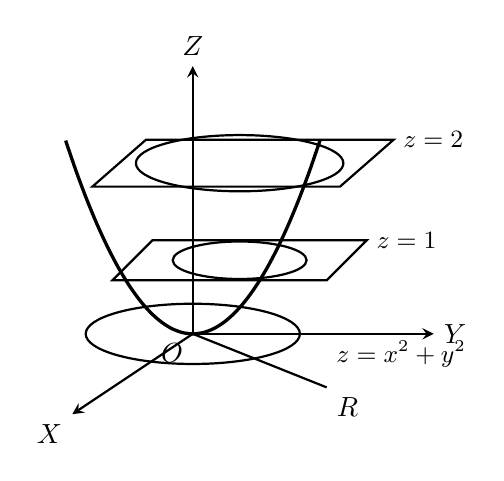
\begin{tikzpicture}[scale=0.85, >=stealth]
  \draw[->, thick] (0, 0) -- (-1.8, -1.2) node[below left] {$X$};
  \draw[->, thick] (0, 0) -- (3.6, 0) node[right] {$Y$};
  \draw[->, thick] (0, 0) -- (0, 4.0) node[above] {$Z$};
  \node[below left] at (0, 0) {$O$};
  
  % Paraboloid outer profile
  \draw[very thick] plot[smooth, domain=-1.9:1.9] (\x, {0.8*\x*\x});
  
  % Level plane z = 1
  \draw[thick] (-1.2, 0.8) -- (2.0, 0.8) -- (2.6, 1.4) -- (-0.6, 1.4) -- cycle;
  \node[right] at (2.6, 1.4) {\small $z = 1$};
  \draw[thick] (0.7, 1.1) ellipse (1.0cm and 0.28cm);
  
  % Level plane z = 2
  \draw[thick] (-1.5, 2.2) -- (2.2, 2.2) -- (3.0, 2.9) -- (-0.7, 2.9) -- cycle;
  \node[right] at (3.0, 2.9) {\small $z = 2$};
  \draw[thick] (0.7, 2.55) ellipse (1.55cm and 0.42cm);
  
  % Base curve in XY plane & Ray OR
  \draw[thick] (0, 0) -- (2.0, -0.8) node[below right] {$R$};
  \draw[thick] (0, 0) ellipse (1.6cm and 0.45cm);
  \node[right] at (2.0, -0.3) {\small $z = x^2 + y^2$};
\end{tikzpicture}
\caption*{(a) 拋物面}
\end{minipage}
\hfill
\begin{minipage}{0.48\textwidth}
\centering
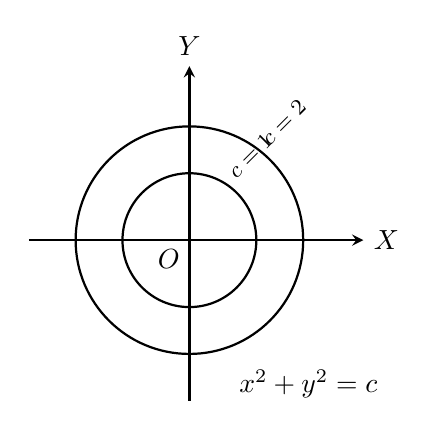
\begin{tikzpicture}[scale=0.85, >=stealth]
  \draw[->, thick] (-2.4, 0) -- (2.6, 0) node[right] {$X$};
  \draw[->, thick] (0, -2.4) -- (0, 2.6) node[above] {$Y$};
  \node[below left] at (0, 0) {$O$};
  
  % Concentric circles
  \draw[thick] (0, 0) circle (1.0cm);
  \node[above right, rotate=45] at (0.7, 0.7) {\footnotesize $c = 1$};
  
  \draw[thick] (0, 0) circle (1.7cm);
  \node[above right, rotate=45] at (1.2, 1.2) {\footnotesize $c = 2$};
  
  \node[below right] at (0.6, -1.8) {$x^2 + y^2 = c$};
\end{tikzpicture}
\caption*{(b) 等溫線系}
\end{minipage}
\caption{拋物面與其等溫線}
\label{fig:b4-ch4-fig4-2}
\end{figure}

\begin{example-non}
【論例 6】 考慮 $z = x^2 - y^2$（雙曲拋物面）．
\end{example-non}

其函數圖形呈一馬鞍狀（如圖 4-3a）．當 $y = 0$ 時函數圖形截於 $z = x^2$ 之開口向上的拋物線，這線成為\textbf{馬脊}；當 $x = 0$ 時函數圖形則截於 $z = -y^2$ 之開口向下的拋物線，這線在\textbf{馬腰}位置．原點 $O$ 稱為一個\textbf{鞍點}．

然後在任一水平面 $z = c$ 上，截函數圖形於 $x^2 - y^2 = c$．此呈一雙曲線，換句話說當水平面自上而下，這些雙曲線掃出一個面；當水平面通過原點 $O$ 時，截得 $x + y = 0, x - y = 0$ 之兩條直線（圖 4-3b）．

\begin{figure}[htbp]
\centering
\begin{minipage}{0.48\textwidth}
\centering
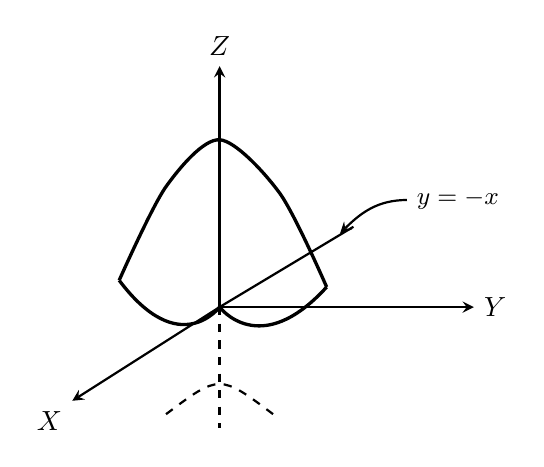
\begin{tikzpicture}[scale=0.85, >=stealth]
  \draw[->, thick] (0, 0) -- (-2.2, -1.4) node[below left] {$X$};
  \draw[->, thick] (0, 0) -- (3.8, 0) node[right] {$Y$};
  \draw[->, thick] (0, 0) -- (0, 3.6) node[above] {$Z$};
  
  % Saddle ridge (upward parabola)
  \draw[very thick] plot[smooth] coordinates {(-1.5, 0.4) (-0.8, 1.8) (0, 2.5) (0.9, 1.7) (1.6, 0.3)};
  % Saddle waist (downward parabolas and wings)
  \draw[very thick] (-1.5, 0.4) .. controls (-0.6, -0.8) and (0, 0) .. (0, 0);
  \draw[very thick] (1.6, 0.3) .. controls (0.6, -0.8) and (0, 0) .. (0, 0);
  \draw[thick, dashed] (0, 0) -- (0, -1.8);
  \draw[thick, dashed] (-0.8, -1.6) .. controls (0, -1.0) .. (0.8, -1.6);
  
  % Asymptote ray with label
  \draw[thick] (0, 0) -- (2.0, 1.2);
  \draw[->, thick] (2.8, 1.6) to[out=180, in=45] (1.8, 1.1);
  \node[right] at (2.8, 1.6) {\small $y = -x$};
\end{tikzpicture}
\caption*{(a) 雙曲拋物面（馬鞍面）}
\end{minipage}
\hfill
\begin{minipage}{0.48\textwidth}
\centering
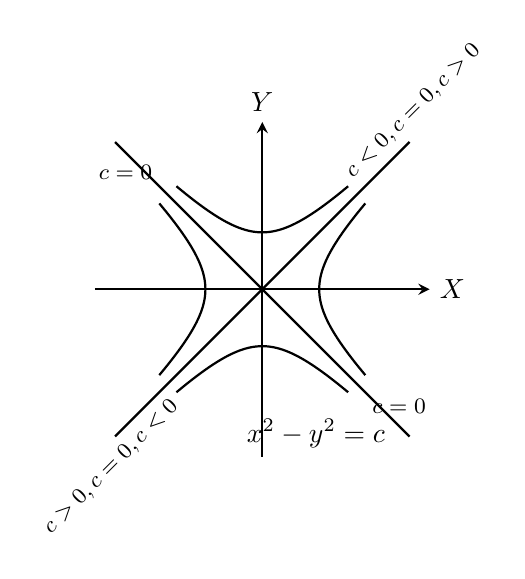
\begin{tikzpicture}[scale=0.85, >=stealth]
  \draw[->, thick] (-2.5, 0) -- (2.5, 0) node[right] {$X$};
  \draw[->, thick] (0, -2.5) -- (0, 2.5) node[above] {$Y$};
  \draw[thick] (-2.2, -2.2) -- (2.2, 2.2);
  \draw[thick] (-2.2, 2.2) -- (2.2, -2.2);
  
  % Hyperbolas c > 0 (left and right)
  \draw[thick] plot[smooth, domain=-1.2:1.2] ({cosh(\x)*0.85}, {sinh(\x)*0.85});
  \draw[thick] plot[smooth, domain=-1.2:1.2] ({-cosh(\x)*0.85}, {sinh(\x)*0.85});
  % Hyperbolas c < 0 (top and bottom)
  \draw[thick] plot[smooth, domain=-1.2:1.2] ({sinh(\x)*0.85}, {cosh(\x)*0.85});
  \draw[thick] plot[smooth, domain=-1.2:1.2] ({sinh(\x)*0.85}, {-cosh(\x)*0.85});
  
  % Labels around asymptotes matching original
  \node[above left] at (-1.5, 1.5) {\footnotesize $c = 0$};
  \node[above right, rotate=45] at (1.4, 1.4) {\footnotesize $c < 0, c = 0, c > 0$};
  \node[below left, rotate=45] at (-1.4, -1.4) {\footnotesize $c > 0, c = 0, c < 0$};
  \node[below right] at (1.5, -1.5) {\footnotesize $c = 0$};
  
  \node[below] at (0.8, -1.8) {$x^2 - y^2 = c$};
\end{tikzpicture}
\caption*{(b) 等溫線系}
\end{minipage}
\caption{雙曲拋物面與等溫線}
\label{fig:b4-ch4-fig4-3}
\end{figure}

\begin{example-non}
【論例 7】 考慮方程式 $x^2 + y^2 - z^2 = 1$．
\end{example-non}

這個三元二次方程式的軌跡可利用二次曲線討論如下：令 $r = \sqrt{x^2 + y^2}$，則方程式化為
\[
r^2 - z^2 = 1
\]
其軌跡在每扇以 $Z$ 軸為軸心的迴轉門上截出雙曲線的一葉．然後將這扇門繞 $Z$ 軸迴轉一圈，此時該葉雙曲線掃出一個\textbf{單葉雙曲面}（圖 4-4）．這雙曲面便應該是原式的軌跡，因在每扇門上它的截痕滿足此式，而此式中的 $r = \sqrt{x^2 + y^2}$．故這雙曲面上的點皆適合．

\begin{figure}[htbp]
\centering
\begin{tikzpicture}[scale=0.85, >=stealth]
  % 3D Axes
  \draw[->, thick] (0, 0) -- (-2.0, -1.3) node[below left] {$X$};
  \draw[->, thick] (0, 0) -- (3.8, 0) node[right] {$Y$};
  \draw[->, thick] (0, 0) -- (0, 3.8) node[above] {$Z$};
  \node[below left] at (0, 0) {$O$};
  
  % Revolving door profile cross-section (with hatching)
  \fill[pattern=north east lines, pattern color=black!30] 
    plot[domain=-1.8:1.8] ({1.1*cosh(0.55*\x)}, \x) -- (0, 1.8) -- (0, -1.8) -- cycle;
  \draw[thick] (0, -1.8) -- (0, 1.8);
  \draw[thick] plot[domain=-1.8:1.8] ({1.1*cosh(0.55*\x)}, \x);
  
  % Left hyperbola boundary
  \draw[very thick] plot[domain=-1.8:1.8] ({-1.1*cosh(0.55*\x)}, \x);
  % Right hyperbola boundary
  \draw[very thick] plot[domain=-1.8:1.8] ({1.1*cosh(0.55*\x)}, \x);
  
  % Top ellipse
  \draw[thick] (0, 1.8) ellipse (1.68cm and 0.42cm);
  % Bottom ellipse
  \draw[thick] (0, -1.8) ellipse (1.68cm and 0.42cm);
  
  % Waist ellipse (z = 0)
  \draw[thick] (0, 0) ellipse (1.1cm and 0.28cm);
\end{tikzpicture}
\caption{單葉雙曲面}
\label{fig:b4-ch4-fig4-4}
\end{figure}

\begin{tcolorbox}[colback=white,colframe=black!60,arc=0mm,boxrule=0.5pt,top=1.5mm,bottom=1.5mm,left=2mm,right=2mm]
\textbf{〔作業 9〕} 試描繪 $z = \dfrac{x^2}{a^2} + \dfrac{y^2}{b^2}$ 之函數圖形，並畫出其相應之「等溫線」系．

\textbf{〔作業 10〕}
\begin{enumerate}[(i)]
  \item 試描繪 $x^2 + y^2 - z^2 = 0$ 之圖形．
  \item 試描繪 $x^2 + y^2 + z^2 = 1$ 之圖形．
\end{enumerate}

\textbf{〔作業 11〕} 利用配方法，證明可取一新座標系 $\bar{S}$ 使 $f(x, y) = x^2 + 2xy + y^2 - 2x + 2y + 1$ 之二次項標準化後化成 $\bar{z} = 2\bar{x}^2 + \dots$，再利用論例 6 的討論描繪其函數圖形．
\end{tcolorbox}

\subsubsection*{乙、\quad 二元二次函數與剛性座標變換}

一個 $x$ 與 $y$ 的二元二次函數
\begin{equation}
f(x, y) = Ax^2 + 2Bxy + Cy^2 + 2Dx + 2Ey + F
\label{eq:b4-ch4-func-fxy}
\end{equation}
可看成是一個 $\mathbb{R}^2 \to \mathbb{R}$ 的變換 $F$ 如下：對 $x \in \mathbb{R}^2$，設 $x$ 的自然座標為 $(x, y)$，則取 $F(x) \in \mathbb{R}$ 之值為
\begin{equation}
F(x) = Ax^2 + 2Bxy + Cy^2 + 2Dx + 2Ey + F.
\label{eq:b4-ch4-fx-val}
\end{equation}

定下來這樣的看法，今取另一正交座標系 $\bar{S} = (O'; \bar{e}_1, \bar{e}_2)$，則 $F(x)$ 用新座標來表示，仍為 $\bar{x}$ 與 $\bar{y}$ 的二元二次函數：
\begin{equation}
\bar{F}(x) = \bar{A}\bar{x}^2 + 2\bar{B}\bar{x}\bar{y} + \bar{C}\bar{y}^2 + 2\bar{D}\bar{x} + 2\bar{E}\bar{y} + \bar{F}
\label{eq:b4-ch4-fbar-val}
\end{equation}
其右端記以 $\bar{f}(\bar{x}, \bar{y})$，此因以剛性座標變換式：
\begin{equation}
\begin{cases}
x = \alpha \bar{x} + \beta \bar{y} + \gamma_1 \\
y = \mp \beta \bar{x} \pm \alpha \bar{y} + \gamma_2
\end{cases}
\label{eq:b4-ch4-rigid-coord-transform}
\end{equation}
代入 \eqref{eq:b4-ch4-fx-val} 式右端之 $x, y$ 即得 $F(x)$（以 $x$ 的新座標成分 $\bar{x}$ 與 $\bar{y}$ 所表示的式子），記以 $\bar{f}(\bar{x}, \bar{y})$，易見其仍為 $\bar{x}, \bar{y}$ 的二次函數（即 \eqref{eq:b4-ch4-fbar-val} 式）．

\begin{definition}
對自然座標系 $S$，記
\[
\delta_S = B^2 - AC, \qquad H_S = A + C, \qquad
\Delta_S = \begin{vmatrix} A & B & D \\ B & C & E \\ D & E & F \end{vmatrix};
\]
而對任一正交座標系 $\bar{S}$，則記
\[
\delta_{\bar{S}} = \bar{B}^2 - \bar{A}\bar{C}, \qquad H_{\bar{S}} = \bar{A} + \bar{C}, \qquad
\Delta_{\bar{S}} = \begin{vmatrix} \bar{A} & \bar{B} & \bar{D} \\ \bar{B} & \bar{C} & \bar{E} \\ \bar{D} & \bar{E} & \bar{F} \end{vmatrix}.
\]
\end{definition}

例如，若 $z = x^2 + y^2 - 2y + 2 = x^2 + (y-1)^2 + 1$，取新座標 $(\bar{x}, \bar{y})_{\bar{S}}$ 使得新舊座標的關係式為：
\[
\begin{cases}
x = \bar{x} \\
y = \bar{y} + 1
\end{cases}
\]
則根據新座標系 $\bar{S}$，新座標之原點 $O'$ 在舊座標 $(0, 1)$ 處（在變換式中代 $\bar{x} = 0, \bar{y} = 0$），而 $\bar{x}^2 + \bar{y}^2$ 為一接觸於 $O'$ 點，且朝上方的拋物面．因此 $\bar{x}^2 + \bar{y}^2 + 1$ 使它提高一單位，而得圖 4-5 之圖形．

\begin{figure}[htbp]
\centering
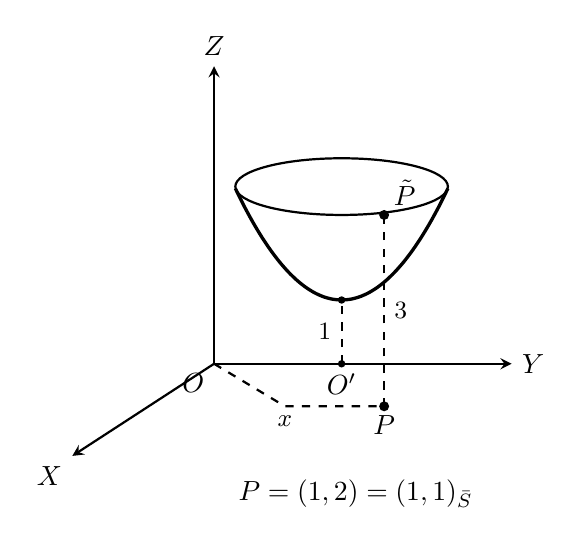
\begin{tikzpicture}[scale=0.9, >=stealth]
  % 3D Axes
  \draw[->, thick] (0, 0) -- (-2.0, -1.3) node[below left] {$X$};
  \draw[->, thick] (0, 0) -- (4.2, 0) node[right] {$Y$};
  \draw[->, thick] (0, 0) -- (0, 4.2) node[above] {$Z$};
  \node[below left] at (0, 0) {$O$};
  
  % Base shift on Y axis to O' in XY plane
  \coordinate (Oprime_base) at (1.8, 0);
  \node[below] at (Oprime_base) {$O'$};
  \fill (Oprime_base) circle (1.5pt);
  
  % Vertex elevated by 1 unit: (0, 1, 1)
  \coordinate (V) at (1.8, 0.9);
  \draw[thick, dashed] (Oprime_base) -- (V) node[midway, left] {\small $1$};
  \fill (V) circle (1.5pt);
  
  % Paraboloid from vertex V
  \draw[very thick] plot[smooth, domain=-1.5:1.5] ({\x + 1.8}, {0.7*\x*\x + 0.9});
  \draw[thick] (1.8, 2.5) ellipse (1.5cm and 0.4cm);
  
  % Point P on XY plane: (1, 2) in old, (1, 1) in new
  \coordinate (P) at (2.4, -0.6);
  \fill (P) circle (2pt) node[below] {$P$};
  \draw[thick, dashed] (0, 0) -- (1.0, -0.6) -- (P);
  \node[below] at (1.0, -0.6) {\small $x$};
  
  % Point \tilde{P} on the paraboloid, z = 3
  \coordinate (Ptilde) at (2.4, 2.1);
  \fill (Ptilde) circle (2pt) node[above right] {$\tilde{P}$};
  \draw[thick, dashed] (P) -- (Ptilde) node[midway, right] {\small $3$};
  
  % Label below
  \node[below] at (2.0, -1.5) {$P = (1, 2) = (1, 1)_{\bar{S}}$};
\end{tikzpicture}
\caption{平移後的拋物面}
\label{fig:b4-ch4-fig4-5}
\end{figure}

設 $x = (1, 2) = (1, 1)_{\bar{S}}$，則
\[
f(1, 2) = 1^2 + 2^2 - 2(2) + 2 = 3, \qquad
\bar{f}(1, 1) = 1^2 + 1^2 + 1 = 3.
\]
兩者皆代表 $P$ 點之 $Z$-座標．

\begin{tcolorbox}[colback=black!5,colframe=black!40,arc=0mm,boxrule=0.5pt,top=1.5mm,bottom=1.5mm,left=2mm,right=2mm]
\textbf{注意：} 上題中，
\[
\delta_S = 0^2 - 1 \cdot 1 = -1, \quad H_S = 1 + 1 = 2, \quad \Delta_S = \begin{vmatrix} 1 & 0 & 0 \\ 0 & 1 & -1 \\ 0 & -1 & 2 \end{vmatrix} = 1.
\]
而
\[
\delta_{\bar{S}} = 0^2 - 1 \cdot 1 = -1, \quad H_{\bar{S}} = 1 + 1 = 2, \quad \Delta_{\bar{S}} = \begin{vmatrix} 1 & 0 & 0 \\ 0 & 1 & 0 \\ 0 & 0 & 1 \end{vmatrix} = 1.
\]
即 $\delta_S = \delta_{\bar{S}}, H_S = H_{\bar{S}}, \Delta_S = \Delta_{\bar{S}}$！
\end{tcolorbox}

我們推知，使 $f(x, y) = 0$ 的點 $P$ 亦使 $\bar{f}(\bar{x}, \bar{y}) = 0$ 反之亦然．故
\begin{align}
Ax^2 + 2Bxy + Cy^2 + 2Dx + 2Ey + F &= 0 \label{eq:b4-ch4-conic-old} \\
\bar{A}\bar{x}^2 + 2\bar{B}\bar{x}\bar{y} + \bar{C}\bar{y}^2 + 2\bar{D}\bar{x} + 2\bar{E}\bar{y} + \bar{F} &= 0 \label{eq:b4-ch4-conic-new}
\end{align}
代表同一條二次曲線．

兩組係數 $\{A, B, C, D, E, F\}$ 與 $\{\bar{A}, \bar{B}, \bar{C}, \bar{D}, \bar{E}, \bar{F}\}$ 間的關係，理論上可由變換式 \eqref{eq:b4-ch4-rigid-coord-transform} 式代入 \eqref{eq:b4-ch4-conic-old} 式左端後與 \eqref{eq:b4-ch4-conic-new} 式左端比較係數而得．一般時候各係數不會相應相等，但上節定理 II 已證明當兩種座標系為同原點時：
\[
\delta = B^2 - AC = \bar{B}^2 - \bar{A}\bar{C} = \bar{\delta}, \qquad
H = A + C = \bar{A} + \bar{C} = \bar{H}.
\]
其詳細道理如下：設 $Q(x, y) = Ax^2 + 2Bxy + Cy^2$，則因將變換式 \eqref{eq:b4-ch4-rigid-coord-transform} 式（此時 $\gamma_1 = \gamma_2 = 0$），即
\[
\begin{cases}
x = \alpha \bar{x} + \beta \bar{y} \\
y = \mp \beta \bar{x} \pm \alpha \bar{y}
\end{cases}
\]
代入 $f(x, y) = Q(x, y) + 2Dx + 2Ey + F$ 中，再經集項成 $\bar{f}(\bar{x}, \bar{y})$ 的一套過程中，所有二次項還是保持不變，換句話說 $Q(x, y) = \bar{Q}(\bar{x}, \bar{y})$．故由上節定理 II，知不變性成立．

實際上，我們更可推出下面的結論：

\begin{theorem}[剛性運動下不變量定理]
設一二次曲線 $\Gamma$ 相關於兩正交座標系 $S = (O; e_1, e_2)$ 與 $\bar{S} = (O'; \bar{e}_1, \bar{e}_2)$ 的軌跡方程式分別為 $f(x, y) = 0$ 與 $\bar{f}(\bar{x}, \bar{y}) = 0$．其中若設 $(x, y)_S$ 與 $(\bar{x}, \bar{y})_{\bar{S}}$ 為同一點 $P$ 的兩種座標使得
\begin{align*}
f(x, y) &= Ax^2 + 2Bxy + Cy^2 + 2Dx + 2Ey + F, \\
\bar{f}(\bar{x}, \bar{y}) &= \bar{A}\bar{x}^2 + 2\bar{B}\bar{x}\bar{y} + \bar{C}\bar{y}^2 + 2\bar{D}\bar{x} + 2\bar{E}\bar{y} + \bar{F},
\end{align*}
則 $\delta, H$ 與 $\Delta$ 為三個基本的不變量，亦即：
\begin{equation}
\begin{aligned}
B^2 - AC &= \bar{B}^2 - \bar{A}\bar{C} \\
A + C &= \bar{A} + \bar{C} \\
\begin{vmatrix} A & B & D \\ B & C & E \\ D & E & F \end{vmatrix} &= \begin{vmatrix} \bar{A} & \bar{B} & \bar{D} \\ \bar{B} & \bar{C} & \bar{E} \\ \bar{D} & \bar{E} & \bar{F} \end{vmatrix}
\end{aligned}
\label{eq:b4-ch4-thm3-invariants}
\end{equation}
\end{theorem}

\begin{proof}
\begin{enumerate}[(i)]
  \item 關於 $\delta$ 與 $H$ 所剩的只是證明它們在平移下的不變性：設 $x = \bar{x} + h, y = \bar{y} + k$，則
  \[
  \begin{aligned}
  &Ax^2 + 2Bxy + Cy^2 + 2Dx + 2Ey + F \\
  &= A(\bar{x} + h)^2 + 2B(\bar{x} + h)(\bar{y} + k) + C(\bar{y} + k)^2 + 2D(\bar{x} + h) + 2E(\bar{y} + k) + F \\
  &= A\bar{x}^2 + 2B\bar{x}\bar{y} + C\bar{y}^2 + 2(Ah + Bk + D)\bar{x} + 2(Bh + Ck + E)\bar{y} + \bar{F}.
  \end{aligned}
  \]
  比較係數得 $\bar{A} = A, \bar{B} = B, \bar{C} = C$．故 $B^2 - AC = \bar{B}^2 - \bar{A}\bar{C}$，且 $A + C = \bar{A} + \bar{C}$．

  \item 至於 $\Delta$，我們也能證明它的不變性．它的證明可直接以座標變換式代入，其計算稍繁；亦可將固有值理論推廣到三度空間中，而證明 $\Delta$ 其實就是三個固有值 $\lambda_1, \lambda_2, \lambda_3$ 的乘積：
  \[
  \Delta = \lambda_1 \lambda_2 \lambda_3 \quad \text{（相當於二度時 $\delta = -\lambda_1 \lambda_2$）}
  \]
  再利用與定理 II 中一樣的討論，證出不變性．
\end{enumerate}

以下我們只解釋這不變性的一部份，我們可根據已有的討論輕易將它說明清楚：定理 I 說二次曲線 $\Gamma$ 的一些特異的幾何型態，如 $\delta \ge 0$ 時 $\Delta_S = 0$ 為其是否特異的判定標準．設取不同的座標系 $\bar{S}$ 所得相應的 $\Delta$ 記為 $\Delta_{\bar{S}}$；則 $\Delta_{\bar{S}} = 0$ 依然是 $\Gamma$ 是否特異的判定標準．但 $\Gamma$ 是否特異不受其方程式所選取的座標表示的影響，故當 $\delta \ge 0$：
\[
\Delta_S = 0 \iff \Gamma \text{ 特異} \iff \Delta_{\bar{S}} = 0.
\]
同樣，但稍為仔細的討論使我們歸結得：
\begin{enumerate}[(i)]
  \item $\Delta_S = 0 \iff \Delta_{\bar{S}} = 0$
  \item 當 $\delta < 0$ 時，$H_S \cdot \Delta_S < 0 \iff H_{\bar{S}} \cdot \Delta_{\bar{S}} < 0$．
\end{enumerate}
\end{proof}

\subsubsection*{習題 IV-4}

求證：
\[
\begin{vmatrix}
a_{11} - \lambda & a_{12} & a_{13} \\
a_{21} & a_{22} - \lambda & a_{23} \\
a_{31} & a_{32} & a_{33} - \lambda
\end{vmatrix} = 0
\]
的根為 $\lambda_1, \lambda_2, \lambda_3$，則
\[
\lambda_1 \lambda_2 \lambda_3 = \begin{vmatrix}
a_{11} & a_{12} & a_{13} \\
a_{21} & a_{22} & a_{23} \\
a_{31} & a_{32} & a_{33}
\end{vmatrix} \quad \text{（行列式值）．}
\]


\subsection{§ IV-5\texorpdfstring{\quad }{ }二次曲線的分類}

本節中我們將利用第二、三節的理論來證明二次曲線的分類定理，亦即在非特異的條件下，二次曲線必為第三章所談過的三種錐線（雙曲線，拋物線，橢圓）之一；並利用不變量 $\delta, \Delta, H$ 來判別其類別．

我們將透過適當的座標變換（旋轉與平移），把一個滿足非特異條件的方程式簡化成第三章討論過的三種標準式．

第三節已經講過，取一同原點的正交座標系 $S = (O; e_1, e_2)$，方程式
\begin{equation}
Ax^2 + 2Bxy + Cy^2 + 2Dx + 2Ey + F = 0
\label{eq:b4-ch4-sec5-conic}
\end{equation}
中的二次項可正性標準化為 $\lambda_1 u^2 + \lambda_2 v^2$，其中 $u, v$ 為點 $P$ 相關於新座標系 $S$ 的座標，且
\[
\begin{cases}
x = \alpha u - \beta v \\
y = \beta u + \alpha v
\end{cases}
\]
式中 $\alpha = \cos\theta, \beta = \sin\theta$．將此代入 \eqref{eq:b4-ch4-sec5-conic} 式，一次項變為：
\[
2Dx + 2Ey = 2D(\alpha u - \beta v) + 2E(\beta u + \alpha v) = 2(D\alpha + E\beta)u + 2(E\alpha - D\beta)v.
\]
故 \eqref{eq:b4-ch4-sec5-conic} 式在新座標系 $S$ 下化為：
\begin{equation}
\lambda_1 u^2 + \lambda_2 v^2 + 2(D\alpha + E\beta)u + 2(E\alpha - D\beta)v + F = 0.
\label{eq:b4-ch4-sec5-rotated}
\end{equation}

\begin{figure}[htbp]
\centering
\begin{tikzpicture}[scale=0.85, >=stealth]
  % Old axes
  \draw[->] (-1.5, 0) -- (3.5, 0);
  \draw[->] (0, -1.2) -- (0, 3.8);
  \node[below left] at (0, 0) {$O$};
  
  % Basis vectors at O
  \draw[->, thick] (0, 0) -- (0.8, 0) node[below=1pt] {$i_1$};
  \draw[->, thick] (0, 0) -- (0, 0.8) node[left=1pt] {$i_2$};
  
  % Rotated basis at O (theta approx 65 deg)
  \def\ang{65}
  \draw[->, thick] (0, 0) -- ({\ang}:1.2) node[right=1pt] {$e_1$};
  \draw[->, thick] (0, 0) -- ({90+\ang}:1.0) node[above left=1pt] {$e_2$};
  
  % Center O'
  \coordinate (Oprime) at (1.8, 2.0);
  \fill (Oprime) circle (1.5pt) node[below right=1pt] {$O'$};
  
  % Major axis line through O' extending past ellipse
  \draw[thick] ($(Oprime) - ({\ang}:2.2)$) -- ($(Oprime) + ({\ang}:2.5)$);
  
  % Vectors from O'
  \draw[->, thick] (Oprime) -- ($(Oprime) + ({\ang}:1.2)$) node[right=1pt] {$e_1$};
  \draw[->, thick] (Oprime) -- ($(Oprime) + ({90+\ang}:1.0)$) node[above left=1pt] {$e_2$};
  
  % Tilted ellipse
  \draw[thick, rotate around={\ang:(Oprime)}] (Oprime) ellipse (1.8cm and 0.85cm);
  
  % Point P
  \coordinate (P) at ($(Oprime) + ({cos(\ang)*1.8*cos(-40) - sin(\ang)*0.85*sin(-40)}, {sin(\ang)*1.8*cos(-40) + cos(\ang)*0.85*sin(-40)})$);
  \fill (P) circle (1.5pt) node[right=2pt] {$P$};
\end{tikzpicture}
\caption{先旋轉後平移的座標幾何}
\label{fig:b4-ch4-fig5-1}
\end{figure}

\paragraph*{(I) 當 $\delta = B^2 - AC = -\lambda_1 \lambda_2 \ne 0$ 時：}
此即 $\lambda_1 \ne 0$ 且 $\lambda_2 \ne 0$．上式可作兩個配方：
\[
\lambda_1 \left( u + \frac{D\alpha + E\beta}{\lambda_1} \right)^2 + \lambda_2 \left( v + \frac{E\alpha - D\beta}{\lambda_2} \right)^2 + F' = 0
\]
其中常數項 $F'$ 滿足 $F' = -\dfrac{\Delta}{\delta}$（作業 14）．

取新原點 $O'\left(-\dfrac{D\alpha + E\beta}{\lambda_1}, -\dfrac{E\alpha - D\beta}{\lambda_2}\right)$ 平移座標系，得：
\begin{equation}
\lambda_1 {u'}^2 + \lambda_2 {v'}^2 + F' = 0.
\label{eq:b4-ch4-sec5-central-std}
\end{equation}
因非特異，故 $\Delta \ne 0 \implies F' \ne 0$．

\begin{itemize}
  \item 若 $\delta > 0$，則 $\lambda_1 \lambda_2 = -\delta < 0$，即 $\lambda_1$ 與 $\lambda_2$ 異號．故 \eqref{eq:b4-ch4-sec5-central-std} 式之軌跡原為一\textbf{雙曲線}．
  \item 若 $\delta < 0$，則 $\lambda_1 \lambda_2 = -\delta > 0$，即 $\lambda_1$ 與 $\lambda_2$ 同號．由非特異假定知 $H\Delta < 0$，兩項與常數項異號，故 \eqref{eq:b4-ch4-sec5-central-std} 式之軌跡為一\textbf{橢圓}．
\end{itemize}

\paragraph*{(II) 當 $\delta = B^2 - AC = -\lambda_1 \lambda_2 = 0$ 時：}
此時恰有一固有值為 0（不妨設 $\lambda_1 = 0, \lambda_2 \ne 0$；不可能 $\lambda_1 = \lambda_2 = 0$，否則 $A = B = C = 0$ 違反二次方程式假定）．則 \eqref{eq:b4-ch4-sec5-rotated} 式成為：
\[
\lambda_2 v^2 + 2(D\alpha + E\beta)u + 2(E\alpha - D\beta)v + F = 0.
\]
經配方後得：
\[
\lambda_2 \left( v + \frac{E\alpha - D\beta}{\lambda_2} \right)^2 + 2(D\alpha + E\beta)u + F'' = 0.
\]
根據非特異假定 $\Delta \ne 0$，可證知 $D\alpha + E\beta \ne 0$．故可經由平移 $u, v$ 座標，將上式化為：
\[
\lambda_2 {v'}^2 + 2(D\alpha + E\beta)u' = 0,
\]
知原式之軌跡為一\textbf{拋物線}．

\begin{theorem}[二次曲線分類定理]
設 $Ax^2 + 2Bxy + Cy^2 + 2Dx + 2Ey + F = 0$ 為一非特異二次曲線，則：
\begin{enumerate}[(1)]
  \item 其軌跡為雙曲線的充要條件是 $\delta > 0$．
  \item 其軌跡為橢圓的充要條件是 $\delta < 0$．
  \item 其軌跡為拋物線的充要條件是 $\delta = 0$．
\end{enumerate}
\end{theorem}

\begin{example-non}
【論例 8】 一非特異的二次曲線，若對稱於原點，則一次項係數等於 0．
\end{example-non}

\begin{proof}
設 $Q(x) \equiv Ax^2 + 2Bxy + Cy^2 + 2Dx + 2Ey + F = 0$ 表一非特異曲線 $\Gamma$．若點 $(x, y)$ 在 $\Gamma$ 上，則由於對稱原點知 $(-x, -y)$ 也必在 $\Gamma$ 上，故
\[
Ax^2 + 2Bxy + Cy^2 - 2Dx - 2Ey + F = 0.
\]
兩式相減得：
\[
4(Dx + Ey) = 0 \implies Dx + Ey = 0.
\]
此表示曲線 $\Gamma$ 落在直線 $Dx + Ey = 0$ 上，與 $\Gamma$ 非特異之假設矛盾！故必有
\[
D = E = 0.
\]
\end{proof}

\begin{figure}[htbp]
\centering
\begin{tikzpicture}[scale=0.85, >=stealth]
  % Axes
  \draw[->] (-1.8, 0) -- (2.2, 0);
  \draw[->] (0, -1.8) -- (0, 2.2);
  
  % 45 degree line L
  \draw (-1.4, -1.4) -- (1.8, 1.8);
  
  % Points (x, y) and (y, x)
  \coordinate (P) at (1.4, 0.4);
  \coordinate (Q) at (0.4, 1.4);
  \coordinate (M) at (0.9, 0.9);
  
  % Connecting segment
  \draw[thick] (P) -- (Q);
  \fill (P) circle (1.5pt) node[right=2pt] {$(x, y)$};
  \fill (Q) circle (1.5pt) node[above=2pt] {$(y, x)$};
  
  % Right angle mark at M
  \draw (M) ++(-0.1, -0.1) -- ++(-0.1, 0.1) -- ++(0.1, 0.1);
  
  % Tick marks on PM and QM
  \draw ($(P)!0.5!(M) + (0.07, 0.07)$) -- ($(P)!0.5!(M) - (0.07, 0.07)$);
  \draw ($(Q)!0.5!(M) + (0.07, 0.07)$) -- ($(Q)!0.5!(M) - (0.07, 0.07)$);
\end{tikzpicture}
\caption{對稱性幾何}
\label{fig:b4-ch4-fig5-2}
\end{figure}

\begin{tcolorbox}[colback=white,colframe=black!60,arc=0mm,boxrule=0.5pt,top=1.5mm,bottom=1.5mm,left=2mm,right=2mm]
\textbf{〔作業 12〕}
\begin{enumerate}[(i)]
  \item 若 $Q(x)$ 非特異，且其圖形對稱 $X$ 軸，則 $y$ 的一次項係數等於 0．
  \item 接上題若其圖形對稱 $Y$ 軸，則 $x$ 的一次項係數等於 0．
  \item 若 $Q(x)$ 對稱於直線 $L: y = x$，則 $A = C, D = E$．〔提示：點 $(x, y)$ 對 $L$ 的鏡點為點 $(y, x)$〕
\end{enumerate}

\textbf{〔作業 13〕} 判斷下列各圖形的對稱性（並求其對稱點或對稱軸）：
\begin{enumerate}[(i)]
  \item $xy = 1$
  \item $2x^2 + y^2 = 0$
  \item $x^2 - y^2 = 1$
\end{enumerate}
\end{tcolorbox}

\begin{example-non}
【論例 9】（有心錐線的心）
\end{example-non}

二次曲線中橢圓和雙曲線因有對稱中心，故稱為\textbf{有心錐線}，其中心的求法如下：

設 $(h, k)$ 為對稱中心，將座標軸平移至 $(h, k)$ 後新座標系為 $x = x' + h, y = y' + k$．展開整理得：
\[
Ax'^2 + 2Bx'y' + Cy'^2 + 2(Ah + Bk + D)x' + 2(Bh + Ck + E)y' + \text{常數項} = 0.
\]
因 $(h, k)$ 為對稱中心，故由論例 8 知 $x', y'$ 兩個一次項的係數等於 0：
\begin{equation}
\begin{cases}
Ah + Bk + D = 0 \\
Bh + Ck + E = 0
\end{cases}
\label{eq:b4-ch4-center-eqs}
\end{equation}
因 $\delta = B^2 - AC \ne 0$，解上聯立方程式可得中心座標：
\[
h = \frac{CD - BE}{\delta}, \qquad k = \frac{AE - BD}{\delta}.
\]
（當 $Q(x)$ 表一拋物線時 $\delta = 0$，聯立方程式無唯一解．）

\begin{tcolorbox}[colback=white,colframe=black!60,arc=0mm,boxrule=0.5pt,top=1.5mm,bottom=1.5mm,left=2mm,right=2mm]
\textbf{〔作業 14〕} 試計算常數項，並證明平移至中心後，常數項 $= -\dfrac{\Delta}{\delta}$．\\
〔提示：常數項 $= Ah^2 + 2Bhk + Ck^2 + 2Dh + 2Ek + F = (Ah+Bk+D)h + (Bh+Ck+E)k + (Dh+Ek+F) = Dh + Ek + F$〕．
\end{tcolorbox}

\begin{example}
判斷 $5x^2 + 8xy + 5y^2 - 18x - 18y + 9 = 0$ 之類別，並化成標準式．
\end{example}

\begin{solution}
$\delta = 4^2 - 5 \times 5 = -9 < 0$．
\[
\Delta = \begin{vmatrix} 5 & 4 & -9 \\ 4 & 5 & -9 \\ -9 & -9 & 9 \end{vmatrix} = -81 < 0.
\]
$H = 5 + 5 = 10 > 0$，故 $H\Delta < 0$，為一\textbf{橢圓}．

由作業 14，知平移至中心後之常數項 $= -\dfrac{\Delta}{\delta} = -\dfrac{-81}{-9} = -9$．

中心座標由 \eqref{eq:b4-ch4-center-eqs} 式求出：
\[
\begin{cases}
5h + 4k - 9 = 0 \\
4h + 5k - 9 = 0
\end{cases}
\implies h = 1, \quad k = 1.
\]
故平移後方程式為 $5{x'}^2 + 8x'y' + 5{y'}^2 - 9 = 0$．

其特徵方程式為
\[
\begin{vmatrix} 5 - \lambda & 4 \\ 4 & 5 - \lambda \end{vmatrix} = 0 \iff (5 - \lambda)^2 - 16 = 0 \iff \lambda^2 - 10\lambda + 9 = 0.
\]
解之得 $\lambda_1 = 9, \lambda_2 = 1$．故再經轉軸後，其標準式可寫成：
\[
9{x''}^2 + {y''}^2 - 9 = 0 \iff \frac{{x''}^2}{1} + \frac{{y''}^2}{9} = 1.
\]
$\lambda = 9$ 相應之單位固有向量為 $e_1 = \left(\dfrac{1}{\sqrt{2}}, \dfrac{1}{\sqrt{2}}\right)$；$\lambda = 1$ 相應之單位固有向量為 $e_2 = \left(-\dfrac{1}{\sqrt{2}}, \dfrac{1}{\sqrt{2}}\right)$（圖 5-3）．
\end{solution}

\begin{figure}[htbp]
\centering
\begin{tikzpicture}[scale=0.85, >=stealth]
  % Axes
  \draw[->] (-1.5, 0) -- (3.2, 0) node[right] {$X$};
  \draw[->] (0, -1.5) -- (0, 3.2) node[above] {$Y$};
  \node[below left] at (0, 0) {$O$};
  
  \coordinate (C) at (1.0, 1.0);
  
  % Shifted axes X', Y'
  \draw[->] ($(C) - (1.3, 0)$) -- ($(C) + (2.0, 0)$) node[right] {$X'$};
  \draw[->] ($(C) - (0, 1.3)$) -- ($(C) + (0, 2.0)$) node[above] {$Y'$};
  \fill (C) circle (1.5pt) node[below right=2pt] {$(1, 1)$};
  
  % Rotated axes X'', Y'' through (1, 1)
  \draw[->] ($(C) - (45:1.8)$) -- ($(C) + (45:2.4)$) node[above right] {$X''$};
  \draw[->] ($(C) - (135:2.4)$) -- ($(C) + (135:2.6)$) node[above left] {$Y''$};
  
  % Basis vectors e_1, e_2
  \draw[->, thick] (C) -- ++(45:0.8) node[right] {$e_1$};
  \draw[->, thick] (C) -- ++(135:0.8) node[above] {$e_2$};
  
  % Ellipse with major axis along 135 deg (length 3) and minor along 45 deg (length 1)
  \draw[thick, rotate around={135:(C)}] (C) ellipse (2.1cm and 0.7cm);
\end{tikzpicture}
\caption{橢圓 $5x^2 + 8xy + 5y^2 - 18x - 18y + 9 = 0$ 之作圖}
\label{fig:b4-ch4-fig5-3}
\end{figure}

\begin{example}
化 $xy = 1$ 為標準式．
\end{example}

\begin{solution}
特徵方程式為
\[
\begin{vmatrix} -\lambda & \frac{1}{2} \\ \frac{1}{2} & -\lambda \end{vmatrix} = 0 \iff \lambda^2 - \frac{1}{4} = 0 \implies \lambda_1 = \frac{1}{2}, \quad \lambda_2 = -\frac{1}{2}.
\]
故其標準式為
\[
\frac{1}{2}{x'}^2 - \frac{1}{2}{y'}^2 = 1 \iff {x'}^2 - {y'}^2 = 2.
\]
此為一等軸雙曲線．$\lambda_1 = \frac{1}{2}$ 相應單位固有向量為 $e_1 = \left(\dfrac{1}{\sqrt{2}}, \dfrac{1}{\sqrt{2}}\right)$；$\lambda_2 = -\frac{1}{2}$ 相應單位固有向量為 $e_2 = \left(-\dfrac{1}{\sqrt{2}}, \dfrac{1}{\sqrt{2}}\right)$（圖 5-4）．
\end{solution}

\begin{figure}[htbp]
\centering
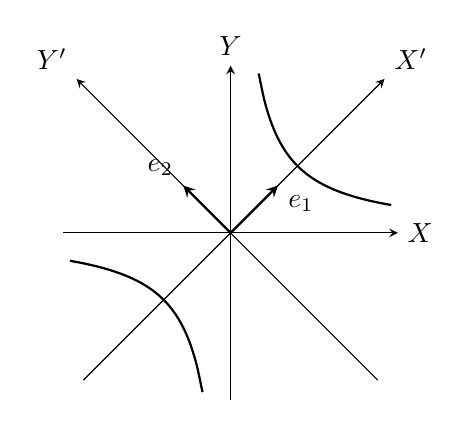
\begin{tikzpicture}[scale=0.85, >=stealth]
  \draw[->] (-2.5, 0) -- (2.5, 0) node[right] {$X$};
  \draw[->] (0, -2.5) -- (0, 2.5) node[above] {$Y$};
  
  % Rotated axes X', Y'
  \draw[->] (-2.2, -2.2) -- (2.3, 2.3) node[above right] {$X'$};
  \draw[->] (2.2, -2.2) -- (-2.3, 2.3) node[above left] {$Y'$};
  
  % Unit vectors e_1, e_2
  \draw[->, thick] (0, 0) -- (45:1.0) node[below right] {$e_1$};
  \draw[->, thick] (0, 0) -- (135:1.0) node[above left] {$e_2$};
  
  % Hyperbola xy = 1
  \draw[thick] plot[smooth, domain=0.42:2.4] (\x, {1/\x});
  \draw[thick] plot[smooth, domain=-2.4:-0.42] (\x, {1/\x});
\end{tikzpicture}
\caption{等軸雙曲線 $xy = 1$}
\label{fig:b4-ch4-fig5-4}
\end{figure}

\begin{tcolorbox}[colback=white,colframe=black!60,arc=0mm,boxrule=0.5pt,top=1.5mm,bottom=1.5mm,left=2mm,right=2mm]
\textbf{〔作業 15〕} 判斷曲線 $7x^2 + 4\sqrt{3}xy + 3y^2 + 18x + 12y + 4 = 0$ 之類別並圖示之．

\textbf{〔作業 16〕} 碰到拋物線的情形，我們無法平移消去一次項，這時只得先求出固有值和固有向量，再利用轉軸消去 $xy$ 項，最後配方繪圖描述．試將 $x^2 + 2xy + y^2 - 2x + 2y - 1 = 0$ 化為標準式並圖示之．
\end{tcolorbox}

\begin{example-non}
【論例 10】（溫度分佈，等溫線及溫度變化最快的方向）
\end{example-non}

假設我們把臺灣地形看成一個平面，來觀察各地溫度情形．現在假設我們以埔里為中心取 1 公里為單位長，正東的方向為 $X$ 軸，正北的方向為 $Y$ 軸，對全省各地做了一次溫度測量：發現點 $(x, y)$ 的溫度是 $t = x^2 + 4y^2$．因此等溫線皆為橢圓，長軸為短軸之 2 倍（圖 5-5）．

我們想由這些等溫線來了解在埔里這點哪個方向溫度變化最大．在以埔里為中心的任一圓內，以 $Y$ 軸方向所截的等溫線最多條．換句話說，和埔里等距離的各個地方中，以正北和正南兩點的溫度最高，故南北向的溫度變化最大．

\begin{figure}[htbp]
\centering
\begin{tikzpicture}[scale=0.85, >=stealth]
  \draw[->] (-3.2, 0) -- (3.2, 0) node[right] {$X$};
  \draw[->] (0, -2.4) -- (0, 2.4) node[above] {$Y$};
  \node[below left] at (0, 0) {$O$};
  
  % Label "埔里" above O inside innermost ellipse
  \node[above=2pt] at (0, 0) {\small 埔里};
  
  % 4 concentric ellipses: horizontal = 2 * vertical
  \draw[thick] (0, 0) ellipse (0.7cm and 0.35cm);
  \draw[thick] (0, 0) ellipse (1.3cm and 0.65cm);
  \draw[thick] (0, 0) ellipse (1.9cm and 0.95cm);
  \draw[thick] (0, 0) ellipse (2.5cm and 1.25cm);
  
  % Circle centered at O
  \draw[thick] (0, 0) circle (1.45cm);
\end{tikzpicture}
\caption{埔里周圍的等溫線系}
\label{fig:b4-ch4-fig5-5}
\end{figure}

\begin{tcolorbox}[colback=white,colframe=black!60,arc=0mm,boxrule=0.5pt,top=1.5mm,bottom=1.5mm,left=2mm,right=2mm]
\textbf{〔作業 17〕} 假設點 $(x, y)$ 的溫度是 $5x^2 - 8xy + 5y^2 + 9$，試繪其等溫線並問在埔里這點溫度的變化以那個方向為最快？
\end{tcolorbox}

\begin{example-non}
【論例 11】（高維空間推廣：三度空間中二次曲面）
\end{example-non}

固有值的理論可以從兩個變數推廣到空間中二次曲面（三度），以至於 $n$ 度空間中，理論的精神和方法完全一致．

試將三元二次式 $7x^2 + 6y^2 + 5z^2 - 4xy - 4yz - 18 = 0$ 化為標準式．

\begin{solution}
其特徵方程式為
\[
\begin{vmatrix}
7 - \lambda & -2 & 0 \\
-2 & 6 - \lambda & -2 \\
0 & -2 & 5 - \lambda
\end{vmatrix} = 0 \iff \lambda^3 - 18\lambda^2 + 99\lambda - 162 = 0.
\]
解之得三根為 $\lambda_1 = 3, \lambda_2 = 6, \lambda_3 = 9$．即原式經過適當的座標變換，可化成
\[
3{x'}^2 + 6{y'}^2 + 9{z'}^2 = 18 \iff \frac{{x'}^2}{6} + \frac{{y'}^2}{3} + \frac{{z'}^2}{2} = 1.
\]
這表示半軸分別為 $\sqrt{6}, \sqrt{3}, \sqrt{2}$ 的\textbf{橢球面}．
\end{solution}

\begin{tcolorbox}[colback=white,colframe=black!60,arc=0mm,boxrule=0.5pt,top=1.5mm,bottom=1.5mm,left=2mm,right=2mm]
\textbf{〔作業 18〕} 將 $2x^2 + 2y^2 + 2z^2 - 2xy - 2yz - 2zx - 1 = 0$ 化為標準式，並從其截痕來看其圖形．
\end{tcolorbox}

\subsubsection*{習題 IV-5}

試判別下列各二次曲線的類別，描其軌跡，定其焦點畫出準線，並繪出其軸（即標準化所根據新座標軸）：
\begin{enumerate}
  \item $x^2 + 4xy + y^2 = 16$.
  \item $x^2 + 6xy + y^2 - 10x - 14y + 9 = 0$.
  \item $3x^2 - 4xy + 8x - 1 = 0$.
  \item $14x^2 - 4xy + 11y^2 - 88x + 34y + 149 = 0$.
  \item $x^2 + 2\sqrt{3}xy + 3y^2 + 6x + 9y + 9 = 0$.
  \item \textbf{（橢圓二次式的特性）} 試證一個二元二次式 $Q(x, y) = Ax^2 + 2Bxy + Cy^2$ 為橢圓二次式的充要條件為 $Q(x, y)$ 為正定或負定．
  
  \textbf{定義：} $Q(x, y) = Ax^2 + 2Bxy + Cy^2$ 稱為橢圓二次式，若 $B^2 - AC < 0$．又若 $Q(x, y) > 0, \forall (x, y) \ne (0, 0)$，則稱 $Q(x, y)$ 為正定；而若 $Q(x, y) < 0, \forall (x, y) \ne (0, 0)$，則稱 $Q(x, y)$ 為負定．
\end{enumerate}


\subsection{*§ IV-6\texorpdfstring{\quad }{ }五點決定一個二次曲線}

我們知道兩點決定一直線（亦即已知平面上相異兩點，有唯一的直線通過這兩點），三點決定一圓．換句話說，在平面上想求一曲線，通過已知（相異的）三點，且這曲線規定是要成一圓；則當這三點不共線時，我們可以找到這樣的圓，而且它是唯一的\phantomsection\label{note:b4-ch4-three-points-circle}\footnote{【原書註記】：若把直線看成圓的特別情形，則不需規定三點不共線，因直線可視為半徑為無限大的圓．}．但如果問題換成「在平面上想求一條曲線通過已知一些點，而規定這曲線是一條二次曲線，則這些已知點的個數究竟一般應為若干，才能使所求的二次曲線存在而且唯一？」我們的結論將是：
\begin{center}
\textbf{「五點決定一二次曲線」}
\end{center}

如果規定該二次曲線成一拋物線，則四點足夠，我們簡稱「四點決定一拋物線」．至於橢圓或雙曲線雖知所屬，我們仍需五點才能決定．這個區別從「拋物線的形狀只須由一個數量便能決定，而橢圓，雙曲線則須兩個數量」的事實中我們可看到一些端倪：拋物線較橢圓或雙曲線易於被決定．

這些道理將伴隨著尋找所求曲線的方法逐一闡明．

一個一般的二元二次方程式
\begin{equation}
Ax^2 + 2Bxy + Cy^2 + 2Dx + 2Ey + F = 0
\label{eq:b4-ch4-sec6-general}
\end{equation}
中雖有六個係數，但將 \eqref{eq:b4-ch4-sec6-general} 式各係數都除以同一常數後所得方程式仍代表同一二次曲線，因此我們要決定的其實是這六個係數間的比例．例如當 $F \ne 0$ 時，\eqref{eq:b4-ch4-sec6-general} 式可皆除以 $F$ 得：
\begin{equation}
\bar{A}x^2 + 2\bar{B}xy + \bar{C}y^2 + 2\bar{D}x + 2\bar{E}y + 1 = 0
\label{eq:b4-ch4-sec6-normalized}
\end{equation}
其中 $\bar{A} = \dfrac{A}{F}, \bar{B} = \dfrac{B}{F}$ 等．這告訴我們二次曲線要決定的係數實際上只有 $\bar{A}, \bar{B}, \bar{C}, \bar{D}, \bar{E}$ 這五個係數，因此理論上，若已知五點 $P_i(x_i, y_i), i=1,2,3,4,5$ 位在這二次曲線上，則因各 $(x_i, y_i)$ 皆能滿足 \eqref{eq:b4-ch4-sec6-general} 式（或 \eqref{eq:b4-ch4-sec6-normalized} 式），分別將它們代入其中得五個方程式，從而決定各係數間的比例，也就決定了這二次曲線本身．

至於實際作法上如何從給定的五個點 $P_i(x_i, y_i)$ 求出通過它們的二次曲線方程式，我們有較簡潔的方法，而不必刻意去解那五個方程式，用下面論例來解釋這個方法：

\begin{example-non}
【論例 12】 求過五點 $P_1(1, -3), P_2(2, -3), P_3(1, 1), P_4(0, 1), P_5(-1, 0)$ 之二次曲線方程式．
\end{example-non}

\begin{solution}
取其中四點 $P_1, P_2, P_3, P_4$．設 $L_{ij}$ 表連結 $P_i$ 與 $P_j$ 兩點的直線，如：
\[
\begin{aligned}
L_{12}&: \frac{y + 3}{x - 1} = \frac{-3 - (-3)}{2 - 1} = 0 \implies y + 3 = 0, \\
L_{34}&: \frac{y - 1}{x - 1} = \frac{1 - 1}{0 - 1} = 0 \implies y - 1 = 0.
\end{aligned}
\]

\begin{figure}[htbp]
\centering
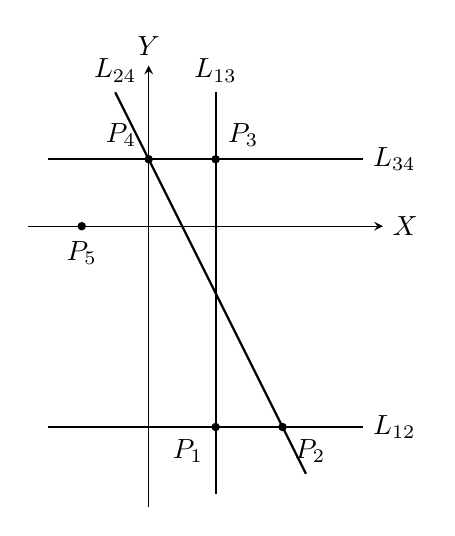
\begin{tikzpicture}[scale=0.85, >=stealth]
  % Axes
  \draw[->] (-1.8, 0) -- (3.5, 0) node[right] {$X$};
  \draw[->] (0, -4.2) -- (0, 2.4) node[above] {$Y$};
  
  % Points
  \coordinate (P1) at (1, -3);
  \coordinate (P2) at (2, -3);
  \coordinate (P3) at (1, 1);
  \coordinate (P4) at (0, 1);
  \coordinate (P5) at (-1, 0);
  
  % Lines
  \draw[thick] (-1.5, -3) -- (3.2, -3) node[right] {$L_{12}$};
  \draw[thick] (-1.5, 1) -- (3.2, 1) node[right] {$L_{34}$};
  \draw[thick] (1, -4.0) -- (1, 2.0) node[above] {$L_{13}$};
  \draw[thick] (-0.5, 2.0) node[above] {$L_{24}$} -- (2.35, -3.7);
  
  % Points markers
  \fill (P1) circle (1.8pt) node[below left=1pt] {$P_1$};
  \fill (P2) circle (1.8pt) node[below right=1pt] {$P_2$};
  \fill (P3) circle (1.8pt) node[above right=1pt] {$P_3$};
  \fill (P4) circle (1.8pt) node[above left=1pt] {$P_4$};
  \fill (P5) circle (1.8pt) node[below=2pt] {$P_5$};
\end{tikzpicture}
\caption{通過四點的二次曲線束}
\label{fig:b4-ch4-fig6-1}
\end{figure}

先求通過 $P_1, P_2, P_3, P_4$ 四點的一個一般二次曲線，想法是作出兩條特別的二次曲線 $\Gamma_1$ 與 $\Gamma_2$ 使其交集為
\[
\Gamma_1 \cap \Gamma_2 = \{ P_1, P_2, P_3, P_4 \}.
\]
然後若 $\Gamma_1: Q_1(x, y) = 0, \Gamma_2: Q_2(x, y) = 0$，則一個通過 $\Gamma_1 \cap \Gamma_2$ 的二次曲線可表成
\begin{equation}
\alpha Q_1(x, y) + \beta Q_2(x, y) = 0.
\label{eq:b4-ch4-sec6-pencil}
\end{equation}
最後再將 $P_5(-1, 0)$ 代入 \eqref{eq:b4-ch4-sec6-pencil} 式，決定出 $\alpha$ 與 $\beta$ 間的比例．

故問題在於先求 $\Gamma_1$ 與 $\Gamma_2$．但注意任兩直線代表一退化的二次曲線．例如 $L_{12}$ 與 $L_{34}$ 的聯集可看成是一個二次曲線，故取
\[
\Gamma_1 = L_{12} \cup L_{34} \implies Q_1(x, y) = (y + 3)(y - 1) = 0.
\]
仍還須求另一也通過 $P_1, P_2, P_3, P_4$ 四點的二次曲線 $\Gamma_2$，很自然我們取 $\Gamma_2 = L_{14} \cup L_{23}$．則因
\[
\begin{aligned}
L_{14}&: \frac{y + 3}{x - 1} = \frac{1 - (-3)}{0 - 1} = -4 \implies 4x + y - 1 = 0, \\
L_{23}&: \frac{y + 3}{x - 2} = \frac{1 - (-3)}{1 - 2} = -4 \implies 4x + y - 5 = 0.
\end{aligned}
\]
故 $\Gamma_2$ 的方程式為 $Q_2(x, y) = (4x + y - 1)(4x + y - 5) = 0$．因此一般通過 $P_1, P_2, P_3, P_4$ 四點的二次曲線方程式可表為：
\begin{equation}
\alpha (y + 3)(y - 1) + \beta (4x + y - 1)(4x + y - 5) = 0.
\label{eq:b4-ch4-sec6-pencil-concrete}
\end{equation}
若要它又通過 $P_5(-1, 0)$ 點，則將 $(-1, 0)$ 代入上式仍應滿足：
\[
\alpha(0 + 3)(0 - 1) + \beta[4(-1) + 0 - 1][4(-1) + 0 - 5] = 0 \implies -3\alpha + 45\beta = 0 \implies \alpha : \beta = 15 : 1.
\]
可取 $\alpha = 15, \beta = 1$ 代回 \eqref{eq:b4-ch4-sec6-pencil-concrete} 式，便是所求．今集項整理得：
\[
2x^2 + xy + 2y^2 - 3x + 3y - 5 = 0.
\]
判別之：
\[
\delta = \left(\frac{1}{2}\right)^2 - 2 \times 2 = -\frac{15}{4} < 0, \qquad
\Delta = \begin{vmatrix} 2 & \frac{1}{2} & -\frac{3}{2} \\ \frac{1}{2} & 2 & \frac{3}{2} \\ -\frac{3}{2} & \frac{3}{2} & -5 \end{vmatrix} = -\frac{81}{8} \ne 0.
\]
且 $H = 2 + 2 = 4 > 0$，故 $H\Delta < 0$，所求為\textbf{橢圓}．
\end{solution}

\begin{tcolorbox}[colback=white,colframe=black!60,arc=0mm,boxrule=0.5pt,top=1.5mm,bottom=1.5mm,left=2mm,right=2mm]
\textbf{〔作業 19〕} 試求經過下面所給定五點的錐線方程式，並判斷其類別：
\begin{enumerate}[(i)]
  \item $P_1(0, 0), P_2(1, 2), P_3(1, -2), P_4(4, 4), P_5(4, -4)$
  \item $P_1(1, 2), P_2(3, 4), P_3(4, 2), P_4(2, -1), P_5(4, 5)$
  \item $P_1(0, 0), P_2(0, 1), P_3(-1, -2), P_4(3, -2), P_5(3, 0)$
\end{enumerate}
\end{tcolorbox}

\begin{example-non}
【論例 13】 求過四點 $P_1(-2, -4), P_2(0, -3), P_3(4, 5), P_4(-6, 0)$ 之拋物線方程式．
\end{example-non}

\begin{solution}
仿上例：
\[
\begin{aligned}
L_{12}&: x - 2y - 6 = 0, \qquad L_{34}: x - 2y + 6 = 0, \\
L_{14}&: x + y + 6 = 0, \qquad L_{23}: 2x - y - 3 = 0.
\end{aligned}
\]
故可設二次曲線方程式為
\[
\alpha(x - 2y - 6)(x - 2y + 6) + \beta(x + y + 6)(2x - y - 3) = 0.
\]
整理二次項得：
\[
(\alpha + 2\beta)x^2 + (\beta - 4\alpha)xy + (4\alpha - \beta)y^2 + \dots = 0.
\]
由拋物線條件 $\delta = 0$：
\[
\left(\frac{\beta - 4\alpha}{2}\right)^2 - (\alpha + 2\beta)(4\alpha - \beta) = 0 \iff \beta(\beta - 4\alpha) = 0.
\]
故得 $\beta = 0$ 或 $\beta = 4\alpha$．將 $\beta = 0$ 代入得兩平行直線 $L_{12} \cup L_{34}$，不為所求．代 $\alpha = 1, \beta = 4$ 則得：
\[
9x^2 - 12xy + 4y^2 + 36x + 12y - 108 = 0 \iff (3x - 2y)^2 + 36x + 12y - 108 = 0
\]
始為所求之拋物線．
\end{solution}

\begin{example-non}
【論例 14】 求通過 $P_1(1, 1), P_2(2, 0), P_3(2, -3)$ 之圓方程式．
\end{example-non}

\begin{solution}
在 § III-5 中我們已經說明可設圓方程式為 $x^2 + y^2 + 2Dx + 2Ey + F = 0$，解聯立方程式求 $D, E, F$．這裡我們要仿照論例 12，13 的做法來決定圓方程式．

過 $P_1$ 點任作一直線 $L': y - 1 - m(x - 1) = 0$．
求直線方程式：
\[
\begin{aligned}
L_{12}&: x + y - 2 = 0, \\
L_{13}&: 4x + y - 5 = 0, \\
L_{23}&: x - 2 = 0.
\end{aligned}
\]
故圓方程式可設為：
\[
\alpha(x + y - 2)(4x + y - 5) + \beta(x - 2)[(y - 1) - m(x - 1)] = 0.
\]
展開比較係數：
\[
\begin{aligned}
x^2 \text{ 項係數}&: 4\alpha - m\beta, \\
y^2 \text{ 項係數}&: \alpha, \\
xy \text{ 項係數}&: 5\alpha + \beta.
\end{aligned}
\]
由圓的條件（$x^2$ 與 $y^2$ 係數相等，且 $xy$ 係數為 0）：
\[
\begin{cases}
4\alpha - m\beta = \alpha \\
5\alpha + \beta = 0
\end{cases}
\implies \beta = -5\alpha, \quad m = -\frac{3}{5}.
\]
代入化簡得方程式為：
\[
x^2 + y^2 + x + 3y - 6 = 0.
\]
\end{solution}

\begin{figure}[htbp]
\centering
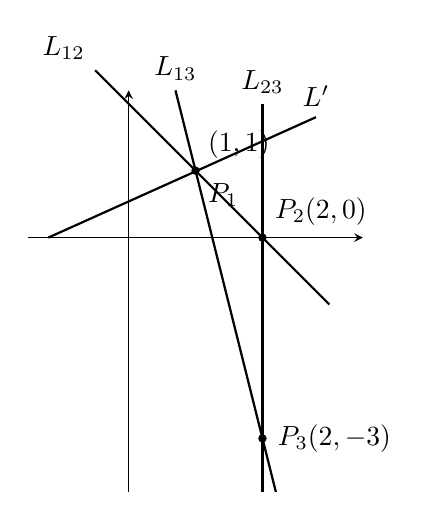
\begin{tikzpicture}[scale=0.85, >=stealth]
  % Axes
  \draw[->] (-1.5, 0) -- (3.5, 0);
  \draw[->] (0, -3.8) -- (0, 2.2);
  
  \coordinate (P1) at (1, 1);
  \coordinate (P2) at (2, 0);
  \coordinate (P3) at (2, -3);
  
  % Lines
  \draw[thick] (-0.5, 2.5) node[above left] {$L_{12}$} -- (3.0, -1.0);
  \draw[thick] (0.7, 2.2) node[above] {$L_{13}$} -- (2.2, -3.8);
  \draw[thick] (2, -3.8) -- (2, 2.0) node[above] {$L_{23}$};
  \draw[thick] (-1.2, 0.0) -- (2.8, 1.8) node[above] {$L'$};
  
  % Points markers
  \fill (P1) circle (1.8pt);
  \node[above right=1pt] at (P1) {$(1,1)$};
  \node[below right=1pt] at (P1) {$P_1$};
  
  \fill (P2) circle (1.8pt);
  \node[above right=1pt] at (P2) {$P_2(2,0)$};
  
  \fill (P3) circle (1.8pt);
  \node[right=2pt] at (P3) {$P_3(2,-3)$};
\end{tikzpicture}
\caption{通過三點決定一圓}
\label{fig:b4-ch4-fig6-2}
\end{figure}


\subsection{*§ IV-7\texorpdfstring{\quad }{ }圓錐面與錐線的再處理}

\begin{tcolorbox}[colback=white,colframe=black!60,arc=0mm,boxrule=0.5pt,top=1.5mm,bottom=1.5mm,left=2mm,right=2mm]
\textbf{〔作業 20〕} 求過 $P_1(0, 1), P_2(3, -2), P_3(5, 0)$ 之圓的方程式．
\end{tcolorbox}

第二章曾以直觀幾何剖析過錐線間之變化情形，在結束這二次曲線的整盤討論之前，我們改以代數性的方法（即座標與向量幾何）來加以申述，澄清其間一些觀念．

\subsubsection*{甲、\quad 從截面來判別錐線類型}

取定一直角座標系 $(O; X, Y, Z)$．

仿第三冊第六章§ VI-4 論例 5 知以 $Z$-軸為固定軸迴轉 $Y$-$Z$ 平面上的兩條直線
\[
\begin{cases}
z = my \\
z = -my
\end{cases}
\quad (0 < m < \infty)
\]
亦即 $z^2 - m^2 y^2 = 0$，得一圓錐面
\[
z^2 - m^2(x^2 + y^2) = 0
\]
亦即
\begin{equation}
x^2 + y^2 = \frac{z^2}{m^2}.
\label{eq:b4-ch4-cone-standard}
\end{equation}

\begin{figure}[htbp]
\centering
\begin{tikzpicture}[scale=0.85, >=stealth]
  \draw[->] (-1.5, 0) -- (3.2, 0) node[right] {$Y$};
  \draw[->] (0, -3.2) -- (0, 3.2) node[above] {$Z$};
  \node[below left] at (0, 0) {$O$};
  
  % Lines z = my and z = -my (slope m approx 2.8)
  \draw[thick] (-1.0, -2.8) -- (1.0, 2.8) node[above right] {$z = my$};
  \draw[thick] (1.0, -2.8) node[below right] {$z = -my$} -- (-1.0, 2.8);
  
  % Angle omega'
  \draw (0, 1.0) arc (90:70.3:1.0);
  \node at (80:1.3) {$\omega'$};
  
  % Slope triangle (y = 0.8)
  \draw[dashed] (0.8, 0) -- (0.8, 2.24);
  \node[below] at (0.8, 0) {$1$};
  \node[right] at (0.8, 1.12) {$m$};
  
  % Cutting plane pi
  \coordinate (M) at (0, -1.2);
  \draw[thick] (-1.6, -2.2) -- (2.4, 0.4) node[above] {平面 $\pi$};
  \fill (M) circle (1.5pt) node[below right=2pt] {$M$};
  
  % Normal vector u (perpendicular to plane pi)
  \draw[->, thick] (M) -- ++(-0.65, -1.0) node[left] {$u$};
  
  % Angle theta with negative Z axis
  \draw (M) ++(0, -0.6) arc (-90:-123:0.6);
  \node at ($(M) + (-0.2, -0.4)$) {$\theta$};
\end{tikzpicture}
\caption{圓錐面與截平面}
\label{fig:b4-ch4-fig7-1}
\end{figure}

這 \eqref{eq:b4-ch4-cone-standard} 式所代表的圓錐面，其中心軸為 $Z$-軸，頂點為座標系的原點 $(0, 0, 0)$；而頂角之半 $\omega'$ 滿足
\begin{equation}
\cos\omega' = \frac{m}{\sqrt{1 + m^2}}, \qquad \sin\omega' = \frac{1}{\sqrt{1 + m^2}}.
\label{eq:b4-ch4-vertex-angle}
\end{equation}

今有一平面
\begin{equation}
\pi: \alpha x + \beta y + \gamma z + \delta = 0
\label{eq:b4-ch4-cutting-plane}
\end{equation}
與圓錐面相截，我們舉例來說明其截角 $\theta$：

\begin{example-non}
【論例 15】 設
\begin{align}
\Omega&: x^2 + y^2 - z^2 = 0 \label{eq:b4-ch4-ex15-cone} \\
\pi&: x + 2y - 2z - 1 = 0 \label{eq:b4-ch4-ex15-plane}
\end{align}
求 $\pi$ 在 $\Omega$ 上截角的正餘弦，而判別其截痕屬於哪種錐線？其離心率若干？
\end{example-non}

\begin{solution}
\begin{enumerate}[(i)]
  \item 設截平面 $\pi$ 與 $\Omega$ 中心軸 $x = y = 0$ 的交點為 $M(0, 0, -1/2)$，$u = \vec{MN}$ 為 $\pi$ 的一個單位法向量使 $N$ 與頂點 $K(0, 0, 0)$ 居於 $\pi$ 的同側，則
  \[
  u = \pm \frac{1}{3}(1, 2, -2) \quad \text{〔取 \eqref{eq:b4-ch4-ex15-plane} 式中三係數 $1, 2, -2$〕}
  \]
  其中 $\pm$ 應為 $+$ 抑 $-$ 將由 $N$ 與 $K$ 同側來決定，方法如下：
  
  與直線分隔平面的情形一樣，平面 $\pi: x + 2y - 2z - 1 = 0$ 將空間分隔成兩部份，同側的點必使
  \[
  x + 2y - 2z - 1
  \]
  同號．據此來決定 $N$．以 $K(0, 0, 0)$ 代入得 $0 + 0 - 0 - 1 < 0$．故 $N$ 之座標亦應取使上式為負者，亦即取
  \[
  \vec{MN} = -\frac{1}{3}(1, 2, -2).
  \]

  \item 今求其截角 $\theta$ 之正餘弦及離心率：\\
  因 $\vec{MK} = (0, 0, 1/2)$，故
  \[
  \cos\theta = \frac{\vec{MN} \cdot \vec{MK}}{|\vec{MK}|} = \frac{2}{3} \implies \sin\theta = +\sqrt{1 - \left(\frac{2}{3}\right)^2} = \frac{\sqrt{5}}{3}.
  \]
  另一方面 $\Omega$ 頂角 $\omega'$ 此時為 $\dfrac{\pi}{4}$，即 $\sin\omega' = \dfrac{1}{\sqrt{2}}$．故離心率
  \[
  e = \frac{\sin\theta}{\sin\omega'} = \frac{\sqrt{5}/3}{1/\sqrt{2}} = \frac{\sqrt{10}}{3} > 1.
  \]

  \item 由其離心率 $e > 1$ 或由 $\theta > \omega'$ 皆可歸結得這截痕為一正類錐線，而由第三章知它是一\textbf{雙曲線}．
\end{enumerate}
\end{solution}

\begin{tcolorbox}[colback=white,colframe=black!60,arc=0mm,boxrule=0.5pt,top=1.5mm,bottom=1.5mm,left=2mm,right=2mm]
\textbf{〔作業 21〕} 設圓錐面 $\Omega: x^2 + y^2 - z^2 = 0$，截平面 $\pi: ax + z - 1 = 0$．求 $\pi$ 在 $\Omega$ 上的截痕的離心率並藉此判別它應屬何種錐線；並求截痕為兩條直線時，$a$ 的條件．
\end{tcolorbox}

\subsubsection*{乙、\quad 截痕為二次曲線的直接驗證}

依照甲段取一直角座標系，將圓錐固定在鉛垂位置，變動平面，要求截痕在此平面上所表成的二元二次方程式，在實際上有相當困難．現在我們從另一個觀點來考慮：\textbf{固定平面為 $XY$-面而讓圓錐變動}，這樣也可得到各色各樣的錐線．道理是要得到不同的截痕，只依賴於圓錐面與截平面的相對位置，盡可任意挑出其中一個予以固定．

設圓錐面 $\Omega$ 之頂點為 $K = (a, b, c)$，沿中心軸之單位向量 $v = (\alpha, \beta, \gamma)$，則一點 $P(x, y, z)$ 在 $\Omega$ 上的充要條件為：
\begin{equation}
\vec{KP} \cdot v = |\vec{KP}| \cos\omega
\label{eq:b4-ch4-cone-vector-def}
\end{equation}

\begin{figure}[htbp]
\centering
\begin{tikzpicture}[scale=0.85, >=stealth]
  % 3D axes
  \draw[->] (0, 0) -- (-1.6, -1.2) node[below left] {$X$};
  \draw[->] (0, 0) -- (3.5, 0) node[right] {$Y$};
  \draw[->] (0, 0) -- (0, 3.2) node[above] {$Z$};
  \node[below left] at (0, 0) {$O$};
  
  % Apex K(a, b, c) and line OK
  \coordinate (K) at (1.8, 1.0);
  \draw (0, 0) -- (K);
  \fill (K) circle (1.5pt) node[below right=1pt] {$K(a, b, c)$};
  
  % Local frame at K
  \draw ($(K) + (0.8, 0.6)$) -- ($(K) - (0.8, 0.6)$);
  \draw ($(K) - (0.6, 0)$) -- ($(K) + (1.2, 0)$);
  \draw (K) -- ($(K) - (0, 0.8)$);
  
  % Cone rim and generators
  \coordinate (Rim) at ($(K) + (0.7, 2.2)$);
  \draw[thick, rotate around={20:(Rim)}] (Rim) ellipse (0.85cm and 0.32cm);
  
  \coordinate (RimL) at ($(Rim) + (-0.8, 0.05)$);
  \coordinate (RimR) at ($(Rim) + (0.8, -0.05)$);
  \draw[thick] (K) -- (RimL);
  \draw[thick] (K) -- (RimR);
  
  % Axis vector v
  \draw[->, thick, dashed] (K) -- ($(K) + (0.45, 1.4)$) node[right=1pt] {$v$};
  
  % Point P on left generator
  \coordinate (P) at ($(K)!0.7!(RimL)$);
  \fill (P) circle (1.5pt) node[above left=1pt] {$P(x, y, z)$};
  \draw[->, thick] (K) -- (P);
  
  % Angle omega arc at K
  \draw (K) ++(0.18, 0.55) arc (72:115:0.5);
  \node at ($(K) + (0.1, 0.7)$) {$\omega$};
  
  % Cone label Omega
  \node at ($(Rim) + (0.6, -0.4)$) {$\Omega$};
\end{tikzpicture}
\caption{任意位置圓錐面的向量幾何}
\label{fig:b4-ch4-fig7-2}
\end{figure}

寫成座標式如下：因 $\vec{KP} = (x - a, y - b, z - c)$，故
\[
[\alpha(x - a) + \beta(y - b) + \gamma(z - c)] = \sqrt{(x - a)^2 + (y - b)^2 + (z - c)^2} \cos\omega
\]
兩邊平方整理後得：
\begin{equation}
[\alpha(x - a) + \beta(y - b) + \gamma(z - c)]^2 - \cos^2\omega [(x - a)^2 + (y - b)^2 + (z - c)^2] = 0.
\label{eq:b4-ch4-cone-general-eq}
\end{equation}
此為圓錐的一般方程式．

今取 $\pi$ 為固定平面 $z = 0$．則將 $z = 0$ 代入 \eqref{eq:b4-ch4-cone-general-eq} 式所得 $x$ 與 $y$ 的二次方程式即為 $\pi$ 在 $\Omega$ 上的截痕．

\begin{example-non}
【論例 16】 設圓錐面 $\Omega$ 的頂點為 $K = (1, 2, 1)$，半頂角皆為 $\omega = \dfrac{\pi}{6}$（$\cos\omega = \dfrac{\sqrt{3}}{2}$），而沿中心軸的單位向量為：
\[
v_1 = \left(0, \frac{1}{\sqrt{2}}, \frac{1}{\sqrt{2}}\right).
\]
求平面 $\pi: z = 0$ 在 $\Omega$ 上的截角，截痕之離心率及其軌跡方程式，並判別其類型．
\end{example-non}

\begin{solution}
先注意 $\pi$ 之單位法向量 $u = (0, 0, 1)$，且 $K(1, 2, 1)$ 與 $u$ 皆指向平面 $z = 0$ 之同側，故截角 $\theta$ 為銳角，得：
\[
\cos\theta = u \cdot v_1 = \frac{1}{\sqrt{2}} \implies \theta = \frac{\pi}{4}.
\]
而頂角之餘角 $\omega' = \frac{\pi}{2} - \omega = \frac{\pi}{2} - \frac{\pi}{6} = \frac{\pi}{3}$．故離心率
\[
e = \frac{\sin\theta}{\sin\omega'} = \frac{1/\sqrt{2}}{\sqrt{3}/2} = \sqrt{\frac{2}{3}} < 1.
\]
故依第二章，截痕 $\Gamma$ 屬負類錐線，即為\textbf{橢圓}．

進一步要求 $\Gamma$ 的軌跡方程式：
\[
\begin{aligned}
\vec{KP} \cdot v_1 &= |\vec{KP}| \cos\omega \\
\implies (x - 1, y - 2, z - 1) \cdot \left(0, \frac{1}{\sqrt{2}}, \frac{1}{\sqrt{2}}\right) &= \frac{\sqrt{3}}{2} \sqrt{(x - 1)^2 + (y - 2)^2 + (z - 1)^2}.
\end{aligned}
\]
將 $\pi: z = 0$ 代入，得 $\Gamma$ 的方程式為：
\[
\frac{1}{\sqrt{2}}(y - 2) + \frac{1}{\sqrt{2}}(-1) = \frac{\sqrt{3}}{2}\sqrt{(x - 1)^2 + (y - 2)^2 + (-1)^2}.
\]
兩端平方得：
\[
2(y - 3)^2 = 3[(x - 1)^2 + (y - 2)^2 + 1].
\]
整理得：
\begin{equation}
3x^2 + y^2 - 6x = 0.
\label{eq:b4-ch4-ex16-ellipse}
\end{equation}

\begin{figure}[htbp]
\centering
\begin{tikzpicture}[scale=0.85, >=stealth]
  % 3D axes
  \draw[->] (0, 0) -- (-1.8, -1.35) node[below left] {$X$};
  \draw[->] (0, 0) -- (3.8, 0) node[right] {$Y$};
  \draw[->] (0, 0) -- (0, 3.2) node[above] {$Z$};
  
  % Ellipse center (1, 0, 0) on X-axis
  \coordinate (C) at (-0.8, -0.6);
  \fill (C) circle (1.5pt) node[below right=2pt] {$(1, 0, 0)$};
  
  % Ellipse on z = 0 plane
  \draw[thick] (C) ellipse (1.8cm and 0.65cm);
  
  % Dimensions on ellipse: \sqrt{3} along Y, 1 along X
  \draw (C) -- ($(C) + (1.2, 0)$);
  \node[above] at ($(C) + (0.6, 0)$) {\small $\sqrt{3}$};
  \node[below left] at ($(C) - (0.5, 0.375)$) {\small $1$};
  
  % Normal vector u
  \draw[->, thick] (C) -- ++(0, 1.4) node[below left=1pt] {$u$};
  
  % Vertex K(1, 2, 1)
  \coordinate (K) at (1.3, 0.9);
  \fill (K) circle (1.5pt) node[below right=1pt] {$K(1, 2, 1)$};
  
  % Lower cone generators to ellipse
  \draw[thick] (K) -- (-2.45, -0.85);
  \draw[thick] (K) -- (0.85, -0.45);
  
  % Upper cone
  \coordinate (RimU) at ($(K) + (1.1, 1.3)$);
  \draw[thick, rotate around={38:(RimU)}] (RimU) ellipse (0.85cm and 0.35cm);
  \draw[thick] (K) -- ($(RimU) + (-0.68, 0.45)$);
  \draw[thick] (K) -- ($(RimU) + (0.68, -0.45)$);
  
  % Axis vector v
  \draw[->, thick] (K) -- ($(K) + (0.7, 0.82)$) node[above=1pt] {$v$};
  
  % Angle arc pi/6
  \draw (K) ++(0.35, 0.41) arc (49:33:0.54);
  \node at ($(K) + (0.6, 0.45)$) {\small $\frac{\pi}{6}$};
  
  % Label Omega
  \node at ($(RimU) + (-0.6, 0.1)$) {$\Omega$};
\end{tikzpicture}
\caption{平面 $z = 0$ 截圓錐面得橢圓}
\label{fig:b4-ch4-fig7-3}
\end{figure}

判別：
\[
\delta = 0 - 3 < 0, \qquad
\Delta = \begin{vmatrix} 3 & 0 & -3 \\ 0 & 1 & 0 \\ -3 & 0 & 0 \end{vmatrix} = -36 < 0, \qquad
H = 3 + 1 = 4 > 0.
\]
故 $H \cdot \Delta < 0$，$\Gamma$ 應為橢圓．

其實只需將 \eqref{eq:b4-ch4-ex16-ellipse} 式配方成準標準式：
\[
3(x - 1)^2 + y^2 = 3 \iff \frac{(x - 1)^2}{1} + \frac{y^2}{3} = 1
\]
即知為平面 $\pi: z = 0$ 上的橢圓，中心在 $(1, 0, 0)$，長短軸半長分別為 $\sqrt{3}$ 與 $1$．
\end{solution}

\begin{tcolorbox}[colback=white,colframe=black!60,arc=0mm,boxrule=0.5pt,top=1.5mm,bottom=1.5mm,left=2mm,right=2mm]
\textbf{〔作業 22〕} 仿此論例作圓錐面沿中心軸單位向量為
\[
v_0 = (0, 0, 1), \qquad
v_2 = \left(0, \frac{\sqrt{3}}{2}, \frac{1}{2}\right), \qquad
v_3 = (0, 1, 0)
\]
的情形，注意四種情形間的演變．
\end{tcolorbox}
